%%%%%%%%%%%%%%%%%%%%%%%%%%%%%%%%%%%%%%%%%
% Wenneker Article
% LaTeX Template
% Version 2.0 (28/2/17)
%
% This template was downloaded from:
% http://www.LaTeXTemplates.com
%
% Authors:
% Vel (vel@LaTeXTemplates.com)
% Frits Wenneker
%
% License:
% CC BY-NC-SA 3.0 (http://creativecommons.org/licenses/by-nc-sa/3.0/)
%
%%%%%%%%%%%%%%%%%%%%%%%%%%%%%%%%%%%%%%%%%

%----------------------------------------------------------------------------------------
%	PACKAGES AND OTHER DOCUMENT CONFIGURATIONS
%----------------------------------------------------------------------------------------

\documentclass[11pt, a4paper]{article} % 10pt font size (11 and 12 also possible), A4 paper (letterpaper for US letter) and two column layout (remove for one column)

\usepackage[english]{babel} % English language hyphenation
\usepackage{microtype} % Better typography
\usepackage{amsmath,amsfonts,amsthm} % Math packages for equations
\usepackage[svgnames]{xcolor,colortbl} % Enabling colors by their 'svgnames'
\usepackage[hang, small, labelfont=bf, up, textfont=it]{caption} % Custom captions under/above tables and figures
\usepackage{booktabs} % Horizontal rules in tables
\usepackage{lastpage} % Used to determine the number of pages in the document (for "Page X of Total")
\usepackage{graphicx} % Required for adding images
\usepackage{amssymb}
\usepackage[mathscr]{eucal}
\usepackage[table]{xcolor}
\usepackage{enumitem} % Required for customising lists
\setlist{noitemsep} % Remove spacing between bullet/numbered list elements
\usepackage{sectsty} % Enables custom section titles
\allsectionsfont{\usefont{OT1}{phv}{b}{n}} % Change the font of all section commands (Helvetica)
\usepackage{hyperref}
\usepackage[sort,numbers]{natbib}
\usepackage{fancyhdr}
\usepackage{url}
\usepackage{floatrow}

\definecolor{Gray}{gray}{0.85}
\definecolor{LightCyan}{rgb}{0.88,1,1}
\definecolor{LightPink}{rgb}{0.25,0.5,1}
\definecolor{bubblegum}{rgb}{0.99, 0.76, 0.8}
\definecolor{pastelpink}{rgb}{1.0, 0.82, 0.86}
\definecolor{piggypink}{rgb}{0.99, 0.87, 0.85}
\definecolor{pink}{rgb}{1, 0.5, 0.9}
\definecolor{lightpink}{rgb}{1.0, 0.61, 0.76}

% ----------------------------------------------------------------------------------------
%	MARGINS AND SPACING
%----------------------------------------------------------------------------------------
\usepackage{geometry} % Required for adjusting page dimensions
\geometry{
	top=1.5cm, % Top margin
	bottom=1.5cm, % Bottom margin
	left=1.5cm, % Left margin
	right=1.5cm, % Right margin
	includehead, % Include space for a header
	includefoot, % Include space for a footer
	%showframe, % Uncomment to show how the type block is set on the page
}
\setlength{\columnsep}{6mm} % Column separation width

%----------------------------------------------------------------------------------------
%	FONTS
%----------------------------------------------------------------------------------------

\usepackage[T1]{fontenc} % Output font encoding for international characters
\usepackage[utf8]{inputenc} % Required for inputting international characters
\usepackage{XCharter} % Use the XCharter font
\usepackage{verbatim} 
%\usepackage{fontspec}
%\setmainfont{TeX Gyre Termes}
\pagestyle{headings}

%%%%%%%%%%%%%%%%%%%%%%%%%%%%%%%%%%%%%%%%%%
% Wenneker Article
% Structure Specification File
% Version 1.0 (28/2/17)
%
% This file originates from:
% http://www.LaTeXTemplates.com
%
% Authors:
% Frits Wenneker
% Vel (vel@LaTeXTemplates.com)
%
% License:
% CC BY-NC-SA 3.0 (http://creativecommons.org/licenses/by-nc-sa/3.0/)
%
%%%%%%%%%%%%%%%%%%%%%%%%%%%%%%%%%%%%%%%%%

%----------------------------------------------------------------------------------------
%	PACKAGES AND OTHER DOCUMENT CONFIGURATIONS
%----------------------------------------------------------------------------------------

\usepackage[english]{babel} % English language hyphenation

\usepackage{microtype} % Better typography

\usepackage{amsmath,amsfonts,amsthm} % Math packages for equations

\usepackage[svgnames]{xcolor} % Enabling colors by their 'svgnames'

\usepackage[hang, small, labelfont=bf, up, textfont=it]{caption} % Custom captions under/above tables and figures

\usepackage{booktabs} % Horizontal rules in tables

\usepackage{lastpage} % Used to determine the number of pages in the document (for "Page X of Total")

\usepackage{graphicx} % Required for adding images

\usepackage{enumitem} % Required for customising lists
\setlist{noitemsep} % Remove spacing between bullet/numbered list elements

\usepackage{sectsty} % Enables custom section titles
\allsectionsfont{\usefont{OT1}{phv}{b}{n}} % Change the font of all section commands (Helvetica)

%----------------------------------------------------------------------------------------
%	MARGINS AND SPACING
%----------------------------------------------------------------------------------------

\usepackage{geometry} % Required for adjusting page dimensions

\geometry{
	top=1cm, % Top margin
	bottom=1.5cm, % Bottom margin
	left=2cm, % Left margin
	right=2cm, % Right margin
	includehead, % Include space for a header
	includefoot, % Include space for a footer
	%showframe, % Uncomment to show how the type block is set on the page
}

\setlength{\columnsep}{7mm} % Column separation width

%----------------------------------------------------------------------------------------
%	FONTS
%----------------------------------------------------------------------------------------

\usepackage[T1]{fontenc} % Output font encoding for international characters
\usepackage[utf8]{inputenc} % Required for inputting international characters

\usepackage{XCharter} % Use the XCharter font

%----------------------------------------------------------------------------------------
%	HEADERS AND FOOTERS
%----------------------------------------------------------------------------------------

\usepackage{fancyhdr} % Needed to define custom headers/footers
\pagestyle{fancy} % Enables the custom headers/footers

\renewcommand{\headrulewidth}{0.0pt} % No header rule
\renewcommand{\footrulewidth}{0.4pt} % Thin footer rule

\renewcommand{\sectionmark}[1]{\markboth{#1}{}} % Removes the section number from the header when \leftmark is used

%\nouppercase\leftmark % Add this to one of the lines below if you want a section title in the header/footer

% Headers
\lhead{} % Left header
\chead{\textit{\thetitle}} % Center header - currently printing the article title
\rhead{} % Right header

% Footers
\lfoot{} % Left footer
\cfoot{} % Center footer
\rfoot{\footnotesize Page \thepage\ of \pageref{LastPage}} % Right footer, "Page 1 of 2"

\fancypagestyle{firstpage}{ % Page style for the first page with the title
	\fancyhf{}
	\renewcommand{\footrulewidth}{0pt} % Suppress footer rule
}

%----------------------------------------------------------------------------------------
%	TITLE SECTION
%----------------------------------------------------------------------------------------

\newcommand{\authorstyle}[1]{{\large\usefont{OT1}{phv}{b}{n}\color{DarkRed}#1}} % Authors style (Helvetica)

\newcommand{\institution}[1]{{\footnotesize\usefont{OT1}{phv}{m}{sl}\color{Black}#1}} % Institutions style (Helvetica)

\usepackage{titling} % Allows custom title configuration

\newcommand{\HorRule}{\color{DarkGoldenrod}\rule{\linewidth}{1pt}} % Defines the gold horizontal rule around the title

\pretitle{
	\vspace{-30pt} % Move the entire title section up
	\HorRule\vspace{10pt} % Horizontal rule before the title
	\fontsize{32}{36}\usefont{OT1}{phv}{b}{n}\selectfont % Helvetica
	\color{DarkRed} % Text colour for the title and author(s)
}

\posttitle{\par\vskip 15pt} % Whitespace under the title

\preauthor{} % Anything that will appear before \author is printed

\postauthor{ % Anything that will appear after \author is printed
	\vspace{10pt} % Space before the rule
	\par\HorRule % Horizontal rule after the title
	\vspace{20pt} % Space after the title section
}

%----------------------------------------------------------------------------------------
%	ABSTRACT
%----------------------------------------------------------------------------------------

\usepackage{lettrine} % Package to accentuate the first letter of the text (lettrine)
\usepackage{fix-cm}	% Fixes the height of the lettrine

\newcommand{\initial}[1]{ % Defines the command and style for the lettrine
	\lettrine[lines=3,findent=4pt,nindent=0pt]{% Lettrine takes up 3 lines, the text to the right of it is indented 4pt and further indenting of lines 2+ is stopped
		\color{DarkGoldenrod}% Lettrine colour
		{#1}% The letter
	}{}%
}

\usepackage{xstring} % Required for string manipulation

\newcommand{\lettrineabstract}[1]{
	\StrLeft{#1}{1}[\firstletter] % Capture the first letter of the abstract for the lettrine
	\initial{\firstletter}\textbf{\StrGobbleLeft{#1}{1}} % Print the abstract with the first letter as a lettrine and the rest in bold
}

%----------------------------------------------------------------------------------------
%	BIBLIOGRAPHY
%----------------------------------------------------------------------------------------

\usepackage[backend=bibtex,style=authoryear,natbib=true]{biblatex} % Use the bibtex backend with the authoryear citation style (which resembles APA)

\addbibresource{example.bib} % The filename of the bibliography

\usepackage[autostyle=true]{csquotes} % Required to generate language-dependent quotes in the bibliography
 % Specifies the document structure and loads requires packages

%----------------------------------------------------------------------------------------
%	ARTICLE INFORMATION
%----------------------------------------------------------------------------------------
\begin{document}
\pagestyle{fancy}
\fancyhf{}
%\fancyhead[LE,RO]{Overleaf}
%\fancyhead[RE,LO]{Guides and tutorials}
%\fancyfoot[LO,RE]{FETOPEN-01 template WP18-20 v20171106}
\fancyfoot[LE,RO]{$\mathcal{ROBHOOT}$}


%\title{$\mathcal{ROBHOOT}$ \\ Open Discovery Network \\ v.1.0}} % The article title
\title{$\mathcal{ROBHOOT}$ \\ Discovery Knowledge Graphs in Biology-Inspired Evolving Federated Networks \\ v.2.0}}
%Automated discovery-knowledge graphs in federated heterogeneous networks
%Evolving Information processing systems in heterogeneous federated networks

%Automated Discovery Knowledge Graphs in Evolving Heterogeneous Federated Networks

%Biology-inspired information processing in large-scale heterogeneous federated networks

%The article title
  %\author{{\textsuperscript{1,2,3} and XY\textsuperscript{2,3}}% Authors
  \newline\newline % Space before institutions
  \\
%	\textsuperscript{1}\institution{}\\ % Institution 1
%	\textsuperscript{2}\institution{}\\ % Institution 2
	%\textsuperscript{3}\institution{\texttt{LaTeXTemplates.com}}
      %} % Institution 3


% Example of a one line author/institution relationship
%\author{\newauthor{John Marston} \newinstitution{Universidad Nacional Autónoma de México, Mexico City, Mexico}}

\date{\today} % Add a date here if you would like one to appear underneath the title block, use \today for the current date, leave empty for no date
%---------------------------------------------------------------------------------------

\maketitle % Print the title
%\thispagestyle{firstpage} % Apply the page style for the first page (no headers and footers)

%----------------------------------------------------------------------------------------
%	ABSTRACT
%----------------------------------------------------------------------------------------
\section*{{\bf Summary}} Global sustainability is a major goal of
humanity. Many studies have shown global sustainability could be
achieved by strengthening transparency, feedbacks and rapid access to
reproducible information among social, ecological, economical,
technological and governance systems. Sustainability goals, however,
strongly depend on global access to evidence-, and discovery-based
knowledge gaps. Yet, science-enabled technologies targeting global
knowledge gaps to reach sustainability goals are at a very incipient
stage of development. We introduce data- and causal-knowledge graphs,
the discovery-knowledge graphs, in federated networks for a
sustainable- and knowledge-inspired society. Discovery-knowledge
graphs running on a federated network encompass a hybrid-technology to
lay out the foundation of an open- and cooperative-science ecosystem
to automate discovery in global emergency and sustainability
challenges. The project summarized here is not set out to deliver
automated discovery-knowledge graphs in federated networks, but to
provide the architecture of a science-enabled technology, as a
proof-of-principle, to connect global human sustainability challenges
to knowledge-inspired societies.
%----------------------------------------------------------------------------------------
%	ARTICLE CONTENTS
% ----------------------------------------------------------------------------------------
\section{Excellence}
\subsection{Radical vision of a science-enabled technology}

\begin{itemize}
\item \textcolor{red}{Describe the vision of a radically-new
    science-enabled technology that the project would contribute
    towards}
\item \textcolor{pink}{The project will contribute towards automated
    discovery-knowledge graphs accounting for heterogeneous
    data-individuals-groups-societies interchanging functional
    information to reach partial solutions in the face of rapidly
    emerging global sustainability challenges.}
\item \textcolor{red}{Describe how this vision surpasses substantially
    any technological paradigms that currently exist or are under
    development.}
\item \textcolor{pink}{Current science-enabled technological paradigms
    are rooted in (single or multiple) optimization functions. Yet,
    biology-inspired technologies targeting learning and cooperation
    in evolving highly heterogeneous systems is currently not in
    place. In addition, technological paradigms for discovery
    targeting global sustainability are currently based on highly
    fragmented, non-reproducible, and competitive
    technologies. Discovery-knowledge graphs in cooperative networks
    instead focus on the need of rapidly responding to global
    sustainability challenges emphasizing learning, cooperation, and
    reproducibility in networks compossed by heterogeneous groups.}
\item \textcolor{red}{Describe the overall and specific objectives for
    the project, which should be clear, measurable, realistic and
    achievable within the duration of the project. (The details of the
    project plan belong to the Implementation section).}
\item \textcolor{pink}{$\mathcal{ROBHOOT}$ will be developed in three
    stages, each containing measurable and achievable goals, work
    packages, milestones and deliverables (Figures 2 and 4 and Tables
    2 and 3).}
\end{itemize}

We are in the midst of the fourth industrial revolution, a
transformation revolving around data driven intelligent machines
potentially impacting strongly knowledge-inspired societies. More than
half of the global population is now online using the Internet (i.e.,
3.9 billion), which represents a more inclusive global information
society ({\bf Ref needed}). ({\bf more flow here}) People are applying
technology in powerful ways, from adopting decentralized technologies
for humanitarian efforts to improving agricultural practices and
reducing waste in the global food supply chain
(\citep{Wilson2018},++). Big Data analytics is advancing at the pace
dictated by the availability of data and a myriad of approaches are
being developed to extract patterns from data (review neural
networks). Most of these approaches focus on a small number of data
sources and groups (refs about heterogeneous and small groups in data
collection). AI approaches are also rapidly evolving towards more
explainable (i.e., interpretable) pattern description making
information about the patterns more accessible (refs). Therefore,
data-driven approaches are built on a few sources of data showing a
quite constrained, but rapidly evolving (refs), number of
interpretable science-enabled technologies ({\bf Maisonobe, M.,
  Eckert, D., Grossetti, M., J�gou, L., & Milard, B. (2016). The world
  network of scientific collaborations between cities: domestic or
  international dynamics?. Journal of Informetrics, 10(4),
  1025-1036}). (this is the gap) In this regard, data collected from
many distinct sources together with science-enabled technologies
accounting for functional interactions among distinct groups making
emphasis on interpretable patterns are required to gain more robust
information access in knowledge-inspired societies. Yet, discovery
science-enabled technologies accounting for fully reproducible
heterogeneous and interpretable data-sources applied to information
access of complex governance, social, environmental and technological
problems are particularly lacking (Figure 1 and Table 1 (remove table
1)) \citep{Mastrangelo2019}.

Taken together, the transformation of a digital society into a
knowledge-inspired society requires solving several gaps: First,
science-enabled technological paradigm assisting humans is biased
towards a limited range of the ``observable'' heterogeneity in
data-sources and therefore a limited number of interpretable patterns
(mention large heterogeneity shown in many datasets, despite they are
only a few data sets). Second, science-enabled technologies mostly
focus on optimization rules (i.e., function loss or reward, similar to
fitness optima functions in evolutionary biology,
refs). Optimization-based technologies limit a broader number of
plausible solutions, as usually found in evolving learning capable
biological systems (refs). Third, science-enabled technologies (for
scientific inquiry) are highly fragmented, partly solve
reproducibility and are mostly developed in close-source software
(\citep{Inhaber1977,Ioannidis2005,Fang2011,Gunther2018,Hardwicke2018,Mehrabi2019,Real2020}). To
leverage the abundance of data, technology should be able to
(automate) data integration from a large number of sources to make it
available for analysis. Second, the analysis of the data should go
beyond the identification of patterns and consider approaches
delivering processes, and the comparison of several processes in an
automated fashion, that is, assisting the end-user. Third, to leverage
the computing capacity the analysis should be performed in federate
way, such that highly heterogeneous populations can learn from each
other to reach consensus about the populations of plausible scenarios
that best capture the properties of the integrated data, and finally,
the whole process should be fully reproducible and transparent such
that benefit the public. (only here we show the vision of a
radically-new science-enabled technology that the project would
contribute towards) Our project contributes towards a science-enabled
technology accounting for massive data heterogeneity and interpretable
patterns, the discovery knowledge graphs (Table 1 and XX), obtained
from evolving learning (neural) information processing systems. (the
dream) Evolutionary learning-inspired technology extracts information
from highly heterogeneous and multidimensional federate networks
minimizing the need of having optimal solutions and making possible
the emergence of functional information processing to reach consensus
about populations of partial solutions to enrich knowledge-inspired
societies facing global challenging problems.

Learning to learn in evolving biological systems have shown multiple
plausible solutions can be obtained all expressing highly
heterogeneous populations (many solutions are not optimal but
suboptimal, maladaptative and require multiple trait dimensions where
some are optimized while other are not, refs). Many branches of
evolutionary algorithms have attempted to capture the patterns and the
mechanisms of the multiple plausible solutions showing functional
communities (evolutionary algorithms, genetic algorithms, the
evolution strategy, evolutionary programming and swarm
intelligence. These techniques form the basis of several disciplines
such as artificial life and evolutionary robotics, refs). On
ecological systems, intraspecific trait variation and trait
dimensionality (i.e., biotic, reproductive, abiotic and migration
traits for example) drive population heterogeneity making difficult to
anticipate functional interactions with other species (i.e.,
cooperative, antagonistic, competitive, or mutualistic, infectious
diseases... etc). (On neural systems, the vast majority of neurons in
the brain show highly differentitated morphological, genetic and
phenotypic states, and making functional interactions among such a
highly differentiatied states (groups, etc) is yet not well
understood.) Taken together, these results show that the understanding
of evolved information processing systems formed by highly
heterogeneous groups (refs about federated networks, bacterial
consortia, federated bacteria..., artificial life, problem solving
artificial societies, and large-scale meta-learning in the federated
setting \citep{Dilley2016}), is currently quite limited and that new
science-enabled approaches accounting for diversification in highly
distinct forms and functions in functional information processing
federated networks, are required to develop science-enabled
technologies ...

Biodiversity dynamics in space and time is a good example of an
evolving information-processing network of interacting species
composed by highly heterogeneous individuals within and between
populations -- a highly heterogeneous mixed pool of evolving
interactions in federated networks (i.e., food webs, mutualistic
networks, hybrid networks, interaction with different types, etc ---
we have expertise in biodiversity and ecological networks -- here to
show more convincingly we are moving beyond our expertise). Many of
these networks are currently loosing species and occur in highly
fragmented and disturbed ecosystems. This makes these systems also
highly vulnerable to the emergence of new interactions many of them
occurring between infectious diseases and humans (i.e., Many zoonosis
have occurred recently with a dramatic rise in global pandemics during
the last decade, i.e., the SARS pandemic in 2003, to Avian Influenza
in 2006, H1N1 in 2009, Ebola in 2014, the appearance of the Zika virus
in Latin America in 2015, and the current Covid-19 pandemic (Zoonosis
from Eating animals or from farms but in any case it is a new and
novel interaction), with these developments inextricably bound up in
modern socio-technical developments and processes of globalization
(Show ++ evidence about the connection between biodiversity loss and
increasing risk of zoonotic diseases -- here enter species
interactions in heterogeneous populations ). Unfortunately,
science-enabled technologies facilitating rapid sharing of data and
information among highly heterogeneous groups to mitigate risks and
enhance global cooperative forecasting to efficiently respond with
informed scenarios are particularly lacking (\citep{Wilson2018}, other
refs). The current pandemic is teaching us the need of science-enabled
technologies facilitating more robust scientific collaboration for
more rapid reaction and real-time interpretable (i.e., causal) maps
accounting for massive data-heterogeneity to overcome fragmented and
partial responses to a global problem. We are responding with many
independent webpages offering data (refs), incipient data-knowledge
graphs (ref), and many epidemiological models with different
assumptions (refs).

All these examples offer an opportunity to build more integrative and
innovative technologies, like the emergence of discovery-knowledge
graphs in ... The goal of $\mathcal{ROBHOOT}$ is to propose a new
hybrid-technology concept integrating data- and causal-knowledge
graphs into intelligent networks to lay the foundation for a novel
scientific discovery technology. $\mathcal{ROBHOOT}$ will contribute
towards facilitating governance reproducible scenarios in rapidly
changing global sustainability landscapes. $\mathcal{ROBHOOT}$ will be
developed along science-enabled technologies (Figures 1, 2, and 4):
{\bf $\mathcal{ROBHOOT}$ v.1.0} deploys question- and data-knowledge
graphs for understanding bias and diversification of information
sources when obtaining global data-architecture maps. {\bf
  $\mathcal{ROBHOOT}$ v.2.0} integrates automated and explainable
biology-inspired neural federated networks to decipher
causal-knowledge graphs from data-knowledge graphs, and {\bf
  $\mathcal{ROBHOOT}$ v.3.0} explores (automated) discovery-knowledge
graphs in federated cooperation networks with a case study mapping the
biodiversity and the risk of zoonosis between humans-infectious
diseases at the global scale.


\begin{figure}[h!]
    \hspace{-0.25 in}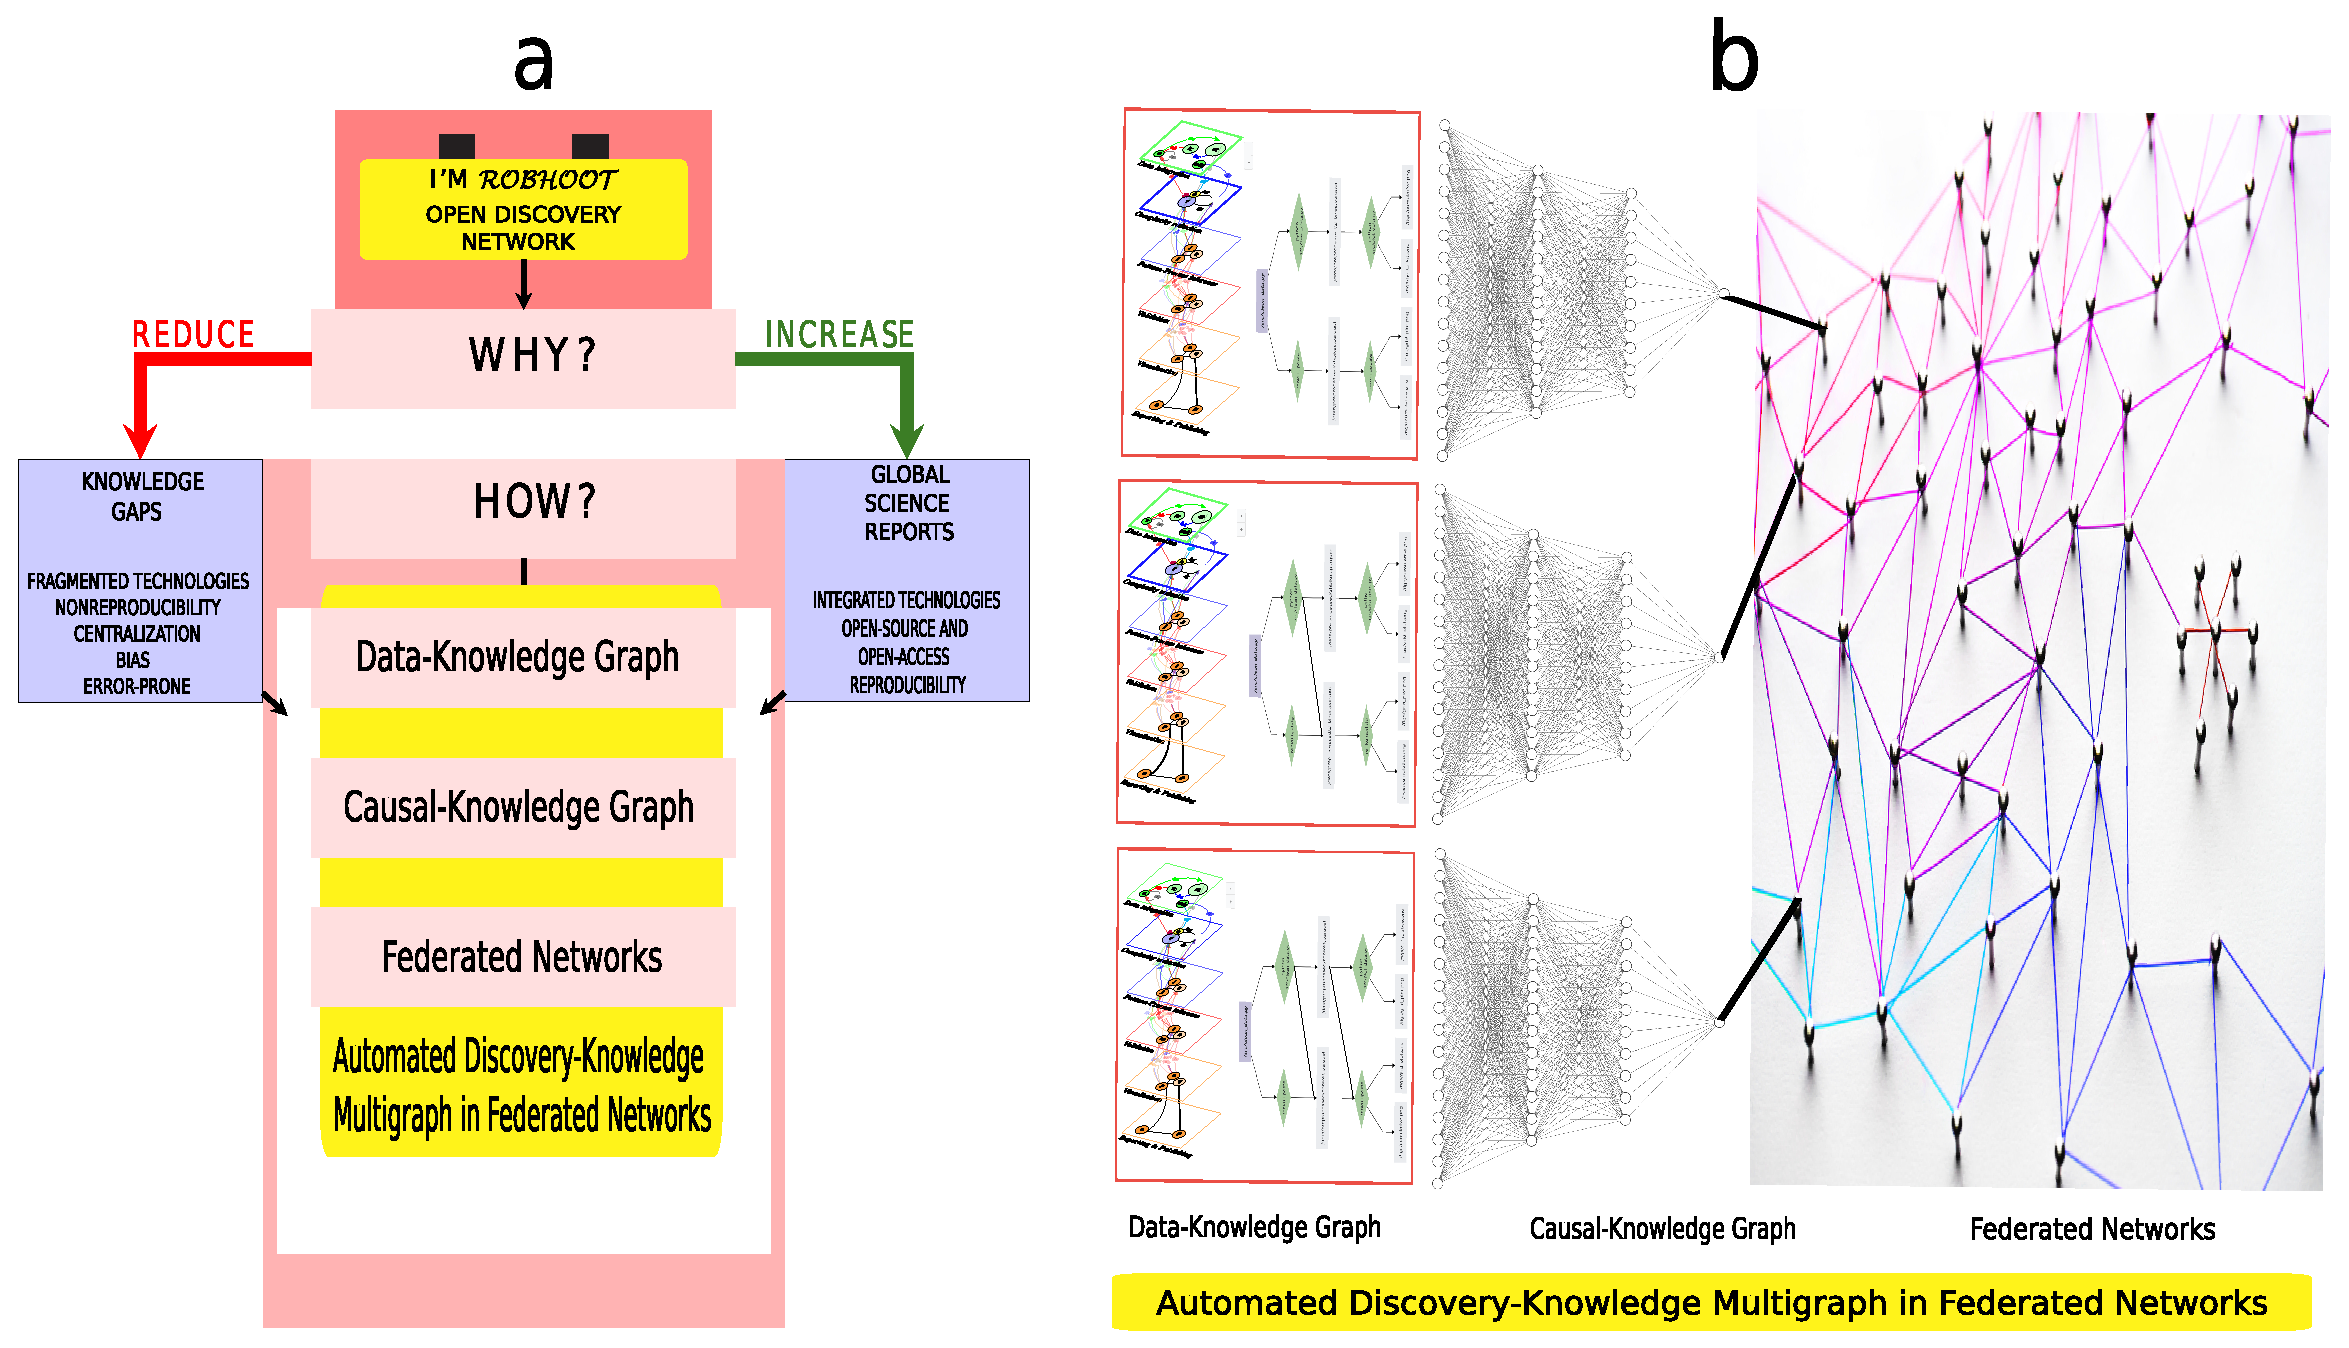
\includegraphics[width=1\textwidth]{Figures/AutomatedDiscovery.pdf}
    \caption*{\small {\bf Figure 1: Cooperative Discovery in Federated
        Networks}. $\mathcal{ROBHOOT}$ integrates data- and
      causal-knowledge graphs, the discovery-knowledge graph, into
      cooperative federated networks for a sustainable
      knowledge-inspired society: {\bf a)} $\mathcal{ROBHOOT}$ targets
      global knowledge gaps (red path) and open-access reproducible
      discovery reports (green path). It integrates three
      science-enabled technologies: {\bf a,b) Data-Knowledge Graphs}
      for discovering global data-architecture. {\bf a,b)
        Causal-Knowledge Graphs} fussion automated and
      explainable biology-inspired neural networks discovery, and {\bf
        a,b) Shared Discovery in Federated Networks} for cooperative
      discovery and forecasting. {\bf Automated Discovery-Knowledge
        Graphs in Federated Networks} integrates data- and
      causal-knowledge graphs into intelligent federated networks to
      generate robust cooperative forecasting to rapidly respond to
      global emergency and sustainability challenges.}}
\end{figure}


%--------------------Currently out of the draft
\begin{comment}
 The Robhoot project is trying to introduce new concepts to allow
  scientist and the public to interact in a decentralized open-access
  knowledge network to gain informed decisions when solving complex
  social, environmental and technological problems. Current
  technologies for scientific inquiry are highly fragmented and thus
  only increase robustness, reproducibility and the interactions with
  the public marginally (refs). The goal of Robhoot is to propose a
  new hybrid-technology concept combining deep learning, automation
  and distributed ledger technology with the advances of neural
  biological networks to lay the foundation for a novel open-science
  ecosystem aiming to couple predictive and knowledge power in
  contemporary societies. Robhoot is not set out to deliver a finished
  deep knowledge ledger network in the science ecosystem but provide a
  science-enabled technology in establishing a prototype
  proof-of-principle for an open public-science ecosystem.
 
\begin{table}
 %\rowcolor{pink}
\begin{tabular}{ p{6cm} | p{3cm} | p{3cm}}
  \hline \hline
  \textbf{Features} & \textbf{Science Ecosystem} &\textbf{{\bf $\mathcal{ROBHOOT}$}}\\  \hline
  Decentralization & No & Yes \\ \hline
  Full automation & No & Yes \\ \hline
  Open-access & Mostly No & Yes \\ \hline
  Immutability & No & Yes \\ \hline
  Robustness & Mostly No & Yes \\ \hline
  Reproducibility & Mostly No & Yes \\ \hline        
  Owner-Controlled assets & No & Yes \\ \hline       
  \bottomrule
\end{tabular}
\caption{{\bf $\mathcal{ROBHOOT}$} is designed to resolve desirable
  properties of science: Open-access, immutability, robustness,
  reproducibility, and owner-controlled assets. These features will be
  added during the different stages of development of the project
  (section ``Design Goals'').}
\end{table}
\end{comment}
%-----------------------------------------------------------------

   
\begin{table*}[ht]
 %\rowcolor{pink}
\begin{tabular}{ p{6cm} | p{11cm}}
  \hline \hline
  \textbf{Word} &\textbf{Meaning}\\  \hline
  Question-knowledge graph & Technology-driven information extraction from corpus or similar to detect question gaps in multidisciplinary research\\ \hline
  Data-knowledge graph & Technology-driven information extraction from diverse data-sources to infer global data-architecture \\ \hline
  Causal-knowledge graph & Technology-driven information extraction to provide explainable/interpretable scenarios on global and complex sustainability challenges\\ \hline
  % Evidence-based knowledge gap & Solid scientific knowledge facing
  % constraints to be transfered to benefit society\\ \hline
  % Research-based knowledge gap & Differential access to the research
  % knowledge limiting information transfer to the society \\ \hline
  Discovery-knowledge graph & Novel interactions emerging from the integration of data- and causal-knowledge graphs to provide multidisciplinary responses to global sustainability challenges\\ \hline
  %Reproducible knowledge graph & High-resolution tracking of the research cycle to make it fully open and transparent\\ \hline
  Automation & Algorithms targeting minimal human-driven interference\\ \hline
  Knowledge-inspired society & Open-access discovery to take informed decisions in global sustainability challenges \\ \hline
  Neutral-knowledge generation & Open reproducible reports making transparent the many sources of bias in the discovery process\\ \hline
  \bottomrule
\end{tabular}
\caption{{\bf Glossary of terms.}}
\end{table*}

\subsection{Science-to-technology breakthrough that addresses this vision}

\begin{itemize}
\item \textcolor{red}{Discuss the relevant state-of-the-art and the
    extent of the advance the project would provide beyond this
    state-of-the-art}
\item \textcolor{pink}{The state-of-the-art of automated and
    interpretable discovery is currently a fragmented landscape. The
    result is a slow response to the rapidly growing global emergency
    and sustainability challenges. $\mathcal{ROBHOOT}$ will go beyond
    the state-of-the-art in automated and interpretable discovery:
    First, it will introduce automated data- and explainable-knowledge
    graphs into a more compact and robust discovery-knowledge graph
    technology. Second, it will fussion the discovery-knowledge graph
    technology within cooperative federated networks to make discovery
    a rapidly evolving feature responding to the also rapidly evolving
    global emergency and sustainability challenges.}
\item \textcolor{red}{Describe the science-to-technology breakthrough,
    targeted by the project that would represent the first proof of
    concept of the envisioned technology.}
\item \textcolor{pink}{Patterns from knowledge-graphs are emerging at
    a fast pace in specific frontiers, but remains isolated from the
    discovery process especially in the context of cooperative
    discovery in federated networks. $\mathcal{ROBHOOT}$ will go
    beyond the state-of-the-art of knowledge-graphs by developing
    data- and causal-knowledge graphs, the discovery-knowledge graphs,
    in cooperative intelligent federated networks to move
    knowledge-inspired societies towards reaching global
    sustainability goals.}
\end{itemize}

\begin{comment}
How does this go beyond the state of the art? Which is the breakthrough?
\end{comment}

Interconnected global societies constantly face new challenges that
need to be rapidly addressed. Yet, technologies integrating
data-driven causal inference into intelligent networks providing rapid
and global interpretable information when solving complex governance,
social, environmental and technological problems are lacking. Depite
rapid advances of research platforms for data analytics in the last
decade
\citep{Melniketal:2010,Steinruecken,Modulos,Guimera2020,GoogleAI,IrisAI,easeml,datarobot,aito},
the integration of science-to-technology intelligent automation
networks currently lack knowledge-inspired technologies impacting
knowledge-inspired societies to help responding to rapidly evolving
global sustainability challenges (Figure 1 and Table 1). In this
regard, technologies facilitating rapid access to global
API-structured data to analyze global data architecture present many
challenges. This is particularly relevant in global emergency or
sustainability landscapes, where data properties like availability,
accuracy and transparency drive constantly emerging feedbacks between
questions and scenarios to predict new situations more accurately.


\textcolor{red}{Redundant -- {\bf $\mathcal{ROBHOOT}$ v.1.0} deploys
  a data discovery technology to generate question- and data-knowledge
  graphs for a rapid understanding of global
  data-architecture. Data-architecture alone is not sufficent to
  outline predictive scenarios in complex sustainability
  problems. Therefore, data analytics complementing data-architecture
  discovery and mechanistic inference is desirable to interpret
  scenarios in rapidly global emerging challenging situations. In this
  regard, there are also many gaps in connecting global
  data-architecture into rapid automated causal-knowledge graphs to
  facilitate discovery that can be transferred to governance
  decisions. {\bf $\mathcal{ROBHOOT}$ v.2.0} integrates automated and
  explainable biology-inspired neural-networks to decipher
  causal-knowledge graphs from open-ended modeling scenarios. Still,
  rapidly drawing scenarios from a few labs limit the phase space from
  where the discovery process is generated. Therefore, the scalability
  of fully reproducible discovery strongly depend on cooperation and
  learning in decentralized networks. {\bf $\mathcal{ROBHOOT}$ v.3.0}
  explores sharing protocols of discovery-knowledge graphs in
  federated networks (section 3.3). Finally, {\bf $\mathcal{ROBHOOT}$
    v.4.0} integrates $\mathcal{ROBHOOT}$ v.1.0 to v.3.0 into
  automated discovery in federated cooperation networks (Figures 2 and
  4).}

\subsection{Interdisciplinarity and non-incrementality of the research
  proposed}

\begin{itemize}
\item \textcolor{red}{Describe the research disciplines necessary for
    achieving the targeted breakthrough of the project and the added
    value from the interdisciplinarity.}
\item \textcolor{red}{Explain why the proposed research is
    non-incremental.}
  \end{itemize}

  \textcolor{red}{Respond more directly -- \\
  {\bf $\mathcal{ROBHOOT}$} is a science-enabled multi-feature
  hybrid-technology for automating interpretable data-driven discovery
  in intelligent and cooperative federated networks (Figures 1 to 4
  and Tables 1 to 3). It will contain four milestones each
  characterized by a mixture of research disciplines necessary for
  achieving interdisciplinary breakthrough. {\bf $\mathcal{ROBHOOT}$
    v.1.0} is compossed by computer scientists and developers
  targeting API discovery protocols and ETLs algorithms. This module
  is complemented with scientists from complex networks to develop
  quantitative methods for question- and data-knowledge graphs to
  decipher the existing gaps in data discovery and data-architecture
  technologies (section 3.1). {\bf $\mathcal{ROBHOOT}$ v.2.0} team is
  compossed by data-scientists trained in deep learning networks and
  automation algorithms, theoreticians and biologists with expertise
  in modeling mechanistic and Bayesian networks and biology-inspired
  neural networks, respectively. The combination of data-scientists,
  theoreticians and biologists will generate a diverse team targeting
  synthesis between automated and explainable biology-inspired
  neural-networks to decipher causal-knowledge graphs from
  data-architecture properties (section 3.2). {\bf $\mathcal{ROBHOOT}$
    v.3.0} is characterized by combining computer scientists and
  developers targeting decentralized protocols (federated networks,
  gnunet), with social scientist, and scientists specialized in
  ecology and evolutionary biology. Team for $\mathcal{ROBHOOT}$ v.3.0
  explores cooperation protocols for discovery in federated networks
  (section 3.3). The complementarity of the teams in modules one to
  three strengthen the collaboration for making $\mathcal{ROBHOOT}$ a
  science-enable functional technology in a rapidly evolving digital
  ecosystem \citep{Soto-Valero2019}. {\bf $\mathcal{ROBHOOT}$ v.4.0}
  combines computer- and data-scientists working in modules one and
  two, respectively, with developers, biologists, evolutionary
  biologists and social scientists working in modules 2 and 3. Such a
  diverse team will integrate automated and explainable data- and
  causal-knowledge graphs into federated cooperation networks to
  generate automated reporting for global emergency and sustainability
  problems (Figure 4).}


 \textcolor{red}{$\mathcal{ROBHOOT}$ aims to bring global transparency in knowledge
  generation by acting as an assistant to humans or as a automated and
  reproducible discovery generator to facilitate sustainability goals
  of humanity. The multi-feature, science-enabled technology target a
  reduction in global knowledge gaps while transparently accounting
  for centralization \citep{Inhaber1977,Gunther2018}⁠⁠, bias⁠⁠
  \citep{Ioannidis2005}, error-prone \citep{Fang2011}, and
  non-reproducibility \citep{Hardwicke2018} (Figure 1 and Table
  1). These features are mostly due to the rapidly evolving digital
  ecosystem. For example, it is increasing continuously its computing
  capacity, new methods intergating automated and explainable AI are
  rapidly advancing, and their interconnection to open-source
  technologies is also rapidly occurring in the digital
  ecosystem. Yet, targeting automated data- and causal-knowledge
  graphs into federated cooperative networks still require the filling
  of many existing technological gaps, from identification and
  retrieval of heterogeneous data sources, to the integration of
  explainable modeling and causal inference and the learning
  capabilities of cooperative forecasting accounting for many evolving
  agents.}

  \begin{comment}
  Yet, technologies with the capacity to compactly accounting for neutral,
  borderless, immutable, and open-access information in hybrid,
  trusted-untrusted peer-to-peer interactions, accounting for the
  multilayer nature of science and engineering are currently not in
  place. We have already advanced in the integration of the different
  modules, from the automated identification, retrieval and data
  integration to inference and process-based discovery. We have
  implemented a prototype for the ongoing covid-19 pandemic (section
  3.3). Each module includes state-of-the-art developments in computer
  science, complex systems, and theoretical evolutionary ecology. The
  proof- of-concept is not fully automated yet and still requires
  human intervention in module integration and the development of a
  testnet stage. Nonetheless, we are currently exploring innovative
  solutions especially in the modules of automated data discovery,
  causal-knowledge graphs, reporting, and visualization.  Producing
  such a technology will require integrating expertise from disparate
  disciplines like multilayer networks, deep learning, automation
  algorithmics, and distributed technologies. The integration of these
  disciplines will require to go beyond domain boundaries.
\end{comment}

%Renku, Fabric and gitchain.

\subsection{High risk, plausibility and flexibility of the research approach}


\begin{itemize}
\item \textcolor{red}{Explain how the research approach relates to the
    project objectives and how it is suitable to deal with the
    considerable science-and-technology uncertainties and appropriate
    for choosing alternative directions and options. (The risks and
    mitigation plan should be spelled out under the Implementation
    section).}
\end{itemize}

\begin{comment}
  Knowledge-inspired societies and governance will demand full
  research cycle transparency, reproducibility and interpretability to
  inform complex social, environmental and technological problems. The
  need of transparency, reproducibility and interpretability brings
  many technical and functional challenges to our research proposal
  because obtaining robust knowledge from integrating many parts each
  containing its own set of methods can generate divergent, fragile
  and contradictory outcomes. {\bf $\mathcal{ROBHOOT}$} will have a
  modular and flexible structure following four main versions each
  divided in four work packages and milestones.
\end{comment}

\begin{comment}
  We will develop a flexible research method focusing more in the
  algorithmic robustness of the deep ledger knowledge network than in
  the development of robust automated knowledge generation. Our
  motivation will be to provide a first proof of concept of how the
  technology works: we will sample the KGs using different deep
  learning algorithms to estimate the uncertainty of the ruled-based
  inference obtained by fitting predictions to simulated data (Goal
  G1). Accounting for the uncertainties of each of the research stages
  when sampling the KGs comes from the many distinct paths within and
  across the layers in the research cycle (Figure 1). We will test a
  variety of consensus algorithms to explore the degree of security,
  decentralization and scalability of the ledger knowledge network
  using the generated population of KGs (Goal G2). Despite our focus
  will be bias towards the side of the algorithmic robustness of the
  deep ledger knowledge network, we will develop a domain-specific
  case study, our Robhoot Open Network, to test the robustness of the
  rule-based inference obtained by fitting each of the generated KG to
  the empirical patterns (Goal G3). The high risk associated to
  robustly automate the full research cycle for producing immutable
  open knowledge is buffered to a great extend because the existing
  ecosystem of tested and reliable open-source tools: We will combine
  our own algorithms (i.e., data integration and deep learning
  algorithms for sampling and automating the KGs) with open-source
  tools like Renku, Fabric and gitchain. This open-ecosystem will
  allow us to have a flexible launching of a testnet to collect data
  to explore the security-scalability-decentralization patterns and
  the robustness of the generated KGs in the deep ledger knowledge
  network (Goal G4.)
\end{comment}



%============IMPACT====================================================
\section{Impact}
\label{cha:impact}


\subsection{Expected impact} 
\label{sec:expected-impact}
\instructions{
  \textit{Please be specific, and provide only information that applies to the proposal and its objectives. Wherever possible, use quantified indicators and targets.}\\
\begin{itemize}
\item \textcolor{red}{Describe how your project will contribute to the
    expected impacts set out in the work programme under the relevant
    topic: Scientific and technological contributions to the
    foundation of a new future technology}
\item \textcolor{pink}{}
\item \textcolor{red}{Describe the importance of the technological
    outcome with regards to its transformational impact on science,
    technology and/or society.}
\item \textcolor{pink}{Decision making and governance at local,
    regional and global scales require access to transparent and
    reproducible data-, and -causal-knowledge graphs, the
    discovery-knowledge graphs, to analyze local solutions benefiting
    society in real-time in emergency situations.}
\item \textcolor{red}{Describe the empowerment of new and high-potential actors
  towards future technological leadership.}
\item \textcolor{red}{Building leading research and innovation
    capacity across Europe by involvement of key actors that can make
    a difference in the future, for example excellent young
    researchers, ambitious high-tech SMEs or first-time participants
    to FET under Horizon 2020}
\item \textcolor{red}{any substantial impacts not mentioned in the
    work programme, that would enhance innovation capacity; create new
    market opportunities, strengthen competitiveness and growth of
    companies, address issues related to climate change or the
    environment, or bring other important benefits for society.}
\item \textcolor{red}{FET Open combines high scientific ambition with
    concrete technological implications. It aims to attract
    interdisciplinary consortia that do not shy away from exploring
    connections between remote disciplines in order to open-up new and
    potentially game changing technological directions that FET as a
    whole aims to develop into the leading technology paradigms of the
    future, including through FET-Proactive projects and FET-Flagship
    initiatives. In spite of the high initial risk, the long-term
    impact can be enormous: these new technologies can become the core
    for new high-growth companies, for new industries or for radically
    new ways of tackling societal challenges.}
\end{itemize}
}

We are moving rapidly towards knowledge-inspired societies in need of
radically tackling new societal and global environmental
challenges. In such a global ecosystem, access to automated
forecasting and interpretable information is key to draw rapid and
robust scenarios when facing complex problems including global
sustainability challenges (i.e., global health, ecosystems
degradation, warming, etc). {\bf $\mathcal{ROBHOOT}$} contributes to
{\bf (evolutionary) automation}, {\bf cooperative forecasting} and
{\bf interpretable information} for a new science-enabled technology
targeting knowledge-inspired societies: First, (evolutionary)
automation decipher open-search interpretation of complex
systems. Second, global hybrid (i.e., humans and machines) cooperative
forecasting challenges existing fragmented responses to emergent
global sustainability problems by compactly offering reproducible
forecasting emerging from many-to-many human and machine cooperative
discovery, and third, open-access explainable information accounts for
global data-arquitecture and causal-knowledge graphs, the
discovery-knowledge graphs, allowing individuals and companies to
access market information to address complex scenarios of future
strategies in highly fluctuating local and global conditions.
Global automated, transparent and reproducible, cooperative, and
explainable discovery can have a large impact to knowledge-inspired
societies in need to access rapid, robust, and reproducible reports to
take informed decisions. It also creates new market opportunities for
companies. First, global-data architecture help to build a vision
about ..., Second,...., and third....

Legal and financial transparency 

Technological Social and Governance 

Impact to emerging and sustainability challenges ::

Novel service for NGO, society and thinktank transparent and
reproducible public policies:

Advisory boards :: 

Sustanaibility -- SDG 

This consortium brings together excellent partners from the fields of
X, Y, Z and technology development, including one SME, who all exhibit
a long-standing experience in interdisciplinary research across the
boundaries of the individual disciplines. The subsection on related
projects shows that this is a novel constellation in Europe (and
possibly world-wide). Thus, this consortium is at the leading edge.


\subsection{Measures to maximize impact} 
\label{sec:maximize-impact}


%mention here the plan for reproducibility and automation
\subsubsection{Dissemination and exploitation of results}
\label{sec:dissemination-exploitation}
\instructions{
\begin{itemize}
\item Provide a plan for disseminating and exploiting the project
  results. The plan, which should be proportionate to the scale of the
  project, should contain measures to be implemented both during and
  after the project.
\item Explain how the proposed measures will help to achieve the
  expected impact of the project.
\item Where relevant, include information on how the participants will
  manage the research data generated and/or collected during the
  project, in particular addressing the following issues:\footnote{For
    further guidance on research data management, please refer to the
    H2020 Online Manual on the Participant Portal.}
\begin{itemize}
\item What types of data will the project generate/collect?
\item What standards will be used?
\item How will this data be exploited and/or shared/made accessible
  for verification and re-use? If data cannot be made available,
  explain why.
\item How will this data be curated and preserved?
\end{itemize}
\emph{You will need an appropriate consortium agreement to manage (amongst other things) the ownership and access to key knowledge (IPR, data etc.). Where relevant, these will allow you, collectively and individually, to pursue market opportunities arising from the project's results.} \\
\emph{The appropriate structure of the consortium to support exploitation is addressed in section 3.3.}\\
\begin{itemize}
\item Outline the strategy for knowledge management and protection. Include measures to provide open access (free on-line access, such as the ``green'' or ``gold'' model) to peer-reviewed scientific publications which might result from the project.\footnote{Open access must be granted to all scientific publications resulting from Horizon 2020 actions. Further guidance on open access is available in the H2020 Online Manual on the Participant Portal.}\\
\end{itemize} 
\emph{Open access publishing (also called 'gold' open access) means that an article is immediately provided in open access mode by the scientific publisher. The associated costs are usually shifted away from readers, and instead (for example) to the university or research institute to which the researcher is affiliated, or to the funding agency supporting the research.}\\
\emph{Self-archiving (also called 'green' open access) means that the
  published article or the final peer-reviewed manuscript is archived
  by the researcher - or a representative - in an online repository
  before, after or alongside its publication. Access to this article
  is often - but not necessarily - delayed (``embargo period''), as
  some scientific publishers may wish to recoup their investment by
  selling subscriptions and charging pay-per-download/view fees during
  an exclusivity period.}
\end{itemize}
}

Strategic dissemination and exploitation will help to explain the
wider societal relevance and long-term economic impact of science,
build support for future research and innovation funding, ensure
uptake of results within the scientific community, open up potential
business opportunities for novel products or services, and potentially
contribute to better decision-making processes and serve as valuable
input for public policies formulation.  Dissemination: General
dissemination targets are scientists, decision-makers, business
community and the public.  General dissemination measures will focus
on project results and stakeholder engagement (stakeholder
consultation processes; workshops to raise awareness, etc.) through:

G1. The project website will be set up within the first three months
of the project.

G2. Up to date information material, e.g. brochures, presentation
slides, will be distributed at events to increase awareness about our
project.

G3. General other publication means will be used such as newspapers,
YouTube, TV and radio, social networks (e.g., Facebook) as well as
targeted mailing lists (e.g., AI-worldwide).

G4. Scientific publications for the scientific community. We will
target high-level journals with open access, like Science, Nature
Communication, etc.

G5. The consortium will visit conferences in the related scientific
fields in order to interactively present and discuss our results with
others. Among other activities, the consortium will organize special
sessions at several conferences.  Additionally, some targeted,
specific dissemination actions will be considered: S1. We need to
address mainly multipliers and developers in the ¿??¿? AI community?¿?
who engage in data processing. This will be achieved by a “traveling
salesman” approach using personal visits and invitations to
demonstrate our system.??  S2. Target groups need to be specified and
addressed.  These are mainly: X departments in relevant companies in
the sectors????  S3. At the end of the project we will organize a
workshop specifically on X?? approaches for disseminating our results
in ??? for assessing future exploitation potential, inviting partners
from academia as well as industry.

1. G4 will launch a testnet to help disseminate the main results of
the deep ledger knowledge network. The launch will have invited NGO’s
and GO across disciplines and social, economical and technological
sectors.

2. The Robhoot Open network will be launched as a Biodiversity
research network to integrate the existing public databases and
crowdsource data collections into the automated KGs and ledger network
to facilitate NGOs, GO and other organizations transparency and
governance in Biodiversity management.

3. The project aims to publish its main findings in top open
scientific journals to communicate the global impact of a deep ledger
knowledge network for transparency and governance across social and
economical sectors.


\subsubsection{Communication activities}
\label{sec:communication}
\instructions{
\begin{itemize}
\item Describe the proposed communication measures for promoting the
  project and its findings during the period of the grant. Measures
  should be proportionate to the scale of the project, with clear
  objectives.  They should be tailored to the needs of various
  audiences, including groups beyond the project's own
  community. Where relevant, include measures for public/societal
  engagement on issues related to the project.
\end{itemize}
}

Data management and accessibility to community:
Other than being constrained by possible IPRs, Robhoot strictly
adheres to the Open Access Policy of the Commission and all
publishable (non-protected) results will follow the green or gold OA
policy. Software as well as hardware protocols will be made openly
available through standard computer science repositories such as
GitHub. Data (measured data), as such, will not be acquired by
Robhoot. Open-source framework for delay analysis Standardized inputs
and software will be made public through an online platform with the
aim of converting it in The Reference Point for any future research in
delay propagation modeling. Open access to publications will be
granted under the terms and conditions laid down in the Grant
Agreement, in accordance with the Rules for participation and
dissemination in Horizon 2020. The beneficiaries will deposit an
electronic copy of the published version or the final manuscript
accepted for publication of a scientific publication relating to
foreground in an institutional or subject-based repository at the
moment of publication, e.g., via the OpenAIRE portal
(www.OpenAIRE.eu). In addition, beneficiaries will make their best
efforts to ensure that this electronic copy becomes freely and
electronically available to anyone through this repository (i.e., that
it becomes “open access”): immediately, if the scientific publication
is published “open access”, i.e., if an electronic version is also
available free of charge via the publisher, or within 6 months of
publication.}

  1. The contribution in communication of the Swiss Data Science Center, Switzerland

  2. Contribution of the Wyss center

  3. Contribution of Ifisc, Spain
%===================END IMPACT======================================

  
\section{Implementation}

\begin{itemize}
\item \textcolor{red}{Describe here the objectives, list of work
    packages, list of deliverables (Ghentt chart)}
\end{itemize}
    
Automating the discovery process to tackle rapid global solutions to
humanity challenges is highly informative by itself, but a diverse
group of scientists across Europe have decided that merely taking
discovery alone is not enough. Science is a highly dynamic and global
process and there are many paths from where it can be achieved. To
understand discovery broadly, these scientists want to advance the
automation and cooperative discovery in the global digital
ecosystem. To this end, the $\mathcal{ROBHOOT}$ consortium aims at
developing a federated network integrating several technologies into a
unified framework. $\mathcal{ROBHOOT}$ will develop quantitative novel
methods such as question-, data-, and causal-knowledge graphs, the
discovery-knowledge graph, to understand how cooperative discovery
networks might help towards knowledge-inspired societies to provide
scenarios in face of global sustainability challenges. This strategy
is expected to improve early access to discovery to rapidly act in
emergency global situations or sustainability challenges to indentify
new emerging targets where automation and global reports can play a
key role in knowledge-inspired societies. $\mathcal{ROBHOOT}$'s goals
are developed in four different stages with four main milestones and
sixteen deliverables (Figure 4).

  
\subsection{Research methodology and work plan – Work packages,
  deliverables}


\subsubsection{{\bf WP1: $\mathcal{ROBHOOT}$ v.1.0}: \\ Data-Knowledge Graphs}

\begin{itemize}
      \item \textcolor{red}{Rapid API access to build
          robust and scalable automated interpretable data-driven
          discovery as an existing need. This is particularly relevant
          in global emergency or sustainability landscapes.}
      \item \textcolor{pink}{Data- and Question-Knowledge graphs as
          solutions for rapid data-driven discovery (Table 1). DKG
          explores similarity patterns of database to discover
          existing gaps in data availability}
      \item \textcolor{red}{Global and rapid API access to build
          robust and scalable question- and data-knowledge graphs as a
          case study for automated interpretable data-driven
          discovery.}
      \item \textcolor{pink}{See Case Study Figure 4}
      \end{itemize}
      
      Global and rapid access to data to build robust and scalable
      question- and data-knowledge graphs is key for automating
      interpretable data-driven discovery. This is particularly needed
      in emergency or sustainability challenging situations at the
      global scale, where new questions and scenarios are constantly
      emerging and data access with different privacy requirements,
      formats, heterogeneity, dimensions, bias and spatiotemporal
      resolution is the norm
      \citep{Openstreetmap,Bluecloud,HOT,Elixir}. Yet, available
      automated science-enabled technologies to build data- and
      question-knowledge graphs to rapidly inform causal-knowledge
      graphs are missing. Fortunately, standard protocols to automate
      data API access, knowledge extraction, and ETFs algorithms are
      rapidly advancing
      \citep{Fan2012,APISGURU,OpenKnowledgeFoundation}, but the
      technologies around automated API data-discovery and question-
      and data-knowledge graphs remain difficult to compactly link to
      the automated causal-knowledge graphs for scientific discovery
      (Table 3.1.1a and 3.1b, Work packages and deliverables).
      
      %Word package description
\begin{table}[h!]
\begin{center}
  \begin{tabular}{|m{3cm} || m{12cm} || m{1cm}|}
    \hline\hline
    \rowcolor{lightpink!30}
    {\bf Work package} & & {\bf Lead Beneficiary} \\
    \hline\hline
    \rowcolor{piggypink!20}
    {\bf Title} & {\bf $\mathcal{ROBHOOT}$ v.1.0} &  \\
    \hline\hline
    \rowcolor{piggypink!20}
    {\bf Participants} & {\bf Fortuna, Egu\'iluz, Choirat} & \\
    \hline\hline
    \rowcolor{piggypink!20}
    {\bf Person Month per participant} & & \\
    \hline\hline
    \rowcolor{piggypink!20}
    {\bf Start month} & {\bf 3} & \\
    \hline\hline
    \rowcolor{piggypink!40}
    {\bf End month} & {\bf 27} & \\
    \hline\hline
    \rowcolor{piggypink!40}
    {\bf Objectives} & Automated Data-Knowledge Graph: Generalized Algorithms and a case study for COVID-19 & \\
    \hline\hline
    \rowcolor{piggypink!40}
    {\bf Description} & $\mathcal{APID}$ $\mathcal{QKG}$ $\mathcal{DKG}$ $\mathcal{CODA}$ & \\
    \hline\hline
    \rowcolor{piggypink!40}
    {\bf Deliverables} & {\bf D1.1: $\mathcal{APID}$}: Technologies around API data-discovery to
                         obtain global knowledge-graphs remain difficult to automate despite
                         standards and protocols are rapidly emerging
                         \citep{Fan2012,APISGURU,OpenKnowledgeFoundation}.
                         \textcolor{red}{{\bf Fortuna}: Check existing protocols and gaps,
                         ODBMS.org and others to build automated knowledge graphs}. Automated workflow to build
                         knowledge-graphs from a large number of API to
                         generate a global data-architecture map.
                         
                         {\bf D1.2: $\mathcal{QKG}$} \textcolor{red}{{\bf Fortuna}:
                         Question-Knowledge graphs from a large number of corpora datasets
                         using automated extraction algorithms. {\bf Choirat}: Convert Question-Knowledge graph into a
                         Reproducible-Knowledge Graph using Renku.}
    
                         {\bf D1.3: $\mathcal{DKG}$} \textcolor{red}{{\bf Fortuna}:
                         Data-Knowledge graphs from a large number of datasets using
                         automated API algorithms. {\bf Egu\'iluz}: Implementation modularity and community metrics to
                         detect gaps in the question-, and data-knowledge graphs. {\bf
                         Choirat}: Encode the Data-Knowledge graph into a
                         Reproducible-Knowledge Graph using Renku.}

                         {\bf D.1.4: $\mathcal{CODA}$}
                         is to produce an Automated Data-Knowledge Graph for the
                         COVID-19, extending the COVID-19 Data-Knowledge Graph built from many
                         data-sources \citep{KGcovid19}. \textcolor{red}{{\bf Fortuna}, {\bf
                         Egu\'iluz}, and {\bf Choirat} generate a reproducible
                         Automated Question- and Data-Knowledge Graph for the COVID-19.} &  \\
    \hline\hline
    \hline\hline
  \end{tabular}
\end{center}
\caption*{{{\bf Table 3.1.1b Work package description}: Work package,
    Title, Participants, Person Months per participant, Start and End
    month, Objectives, Description and deliverables of each Work
    Package.}}
\end{table}


\begin{table}[h!]
\begin{center}
  \begin{tabular}{|m{3cm} || m{12cm} || m{1cm}|}
    \hline\hline
    \rowcolor{lightpink!30}
    {\bf Work package} & & {\bf Lead Beneficiary} \\
    \hline\hline
    \rowcolor{piggypink!20}
    {\bf Title} & {\bf $\mathcal{ROBHOOT}$ v.2.0} &  \\
    \hline\hline
    \rowcolor{piggypink!20}
    {\bf Participants} & {\bf Baity, Guimer\`a, Meli\'an, Vicente} & \\
    \hline\hline
    \rowcolor{piggypink!20}
    {\bf Person Month per participant} & & \\
    \hline\hline
    \rowcolor{piggypink!20}
    {\bf Start month} & {\bf 5} & \\
    \hline\hline
    \rowcolor{piggypink!40}
    {\bf End month} & {\bf 29} & \\
    \hline\hline
    \rowcolor{piggypink!40}
    {\bf Objectives} & Automated Causal-Knowledge Graph: case study for COVID-19 & \\
    \hline\hline
    \rowcolor{piggypink!40}
    {\bf Description} & $\mathcal{EAIA}$ $\mathcal{CKG}$ $\mathcal{BSM}$ $\mathcal{COCAU}$ & \\
    \hline\hline
    \rowcolor{piggypink!40}
    {\bf Deliverables} & {\bf D1.1: $\mathcal{EAIA}$}:
                         Automated evolutionary AI Algorithms with open-ended (evolving) functions with
                         different degrees of complexity to find expressions (i.e., interpretable models towards
                         causal-knowledge graphs) best fitting
                         the empirical patterns observed in the Data-Knowledge Graphs
                         \citep{Guimera2020,Steinruecken}. \textcolor{red}{Merge Evolutionary algorithms (i.e.,,
                         mutation-selection-migration-recombination algorithms
                         ({\bf Meli\'an}, {\bf Guimer\`a}) with deep neural networks
                         ({\bf Baity}, {\bf Vicente}).}
                         
                         {\bf D1.2: $\mathcal{CKG}$} \textcolor{red}{{\bf Baity, Guimer\`a, Meli\'an, Vicente}:
                         Discovery-Knowledge Graphs generated from the fussion of
                         Data-, and Causal-Knowledge graphs (Figure 3) using automated evolutionary
                         AI Algorithms. {\bf Choirat}: Convert Causal-Knowledge graph into a
                         Reproducible-Knowledge Graph using Renku.}
    
                         {\bf D1.3: $\mathcal{BSM}$} \textcolor{red}{{\bf Baity, Guimer\`a, Meli\'an, Vicente}:
                         Bayesian Inference to estimate Causal-Knowledge graphs accounting for model complexity.                          Check link to automated evolutionary AI algorithms via open-ended (evolving) functions.}

                         {\bf D.1.4: $\mathcal{COCAU}$} \textcolor{red}{{\bf Baity, Guimer\`a, Meli\'an, Vicente}
                         Bayesian Inference to estimate Causal-Knowledge graphs accounting for model
                         complexity for the COVID-19 as a case study.
                         Check link to automated evolutionary AI algorithms via open-ended (evolving) functions.} &  \\
    \hline\hline
    \hline\hline
\end{tabular}
\end{center}
\caption*{{{\bf Table 3.1.2b Work package description}: Work package,
    Title, Participants, Person Months per participant, Start and End
    month, Objectives, Description and deliverables of each Work
    Package.}}
\end{table}


 \begin{figure}[h!]
  %\centering
   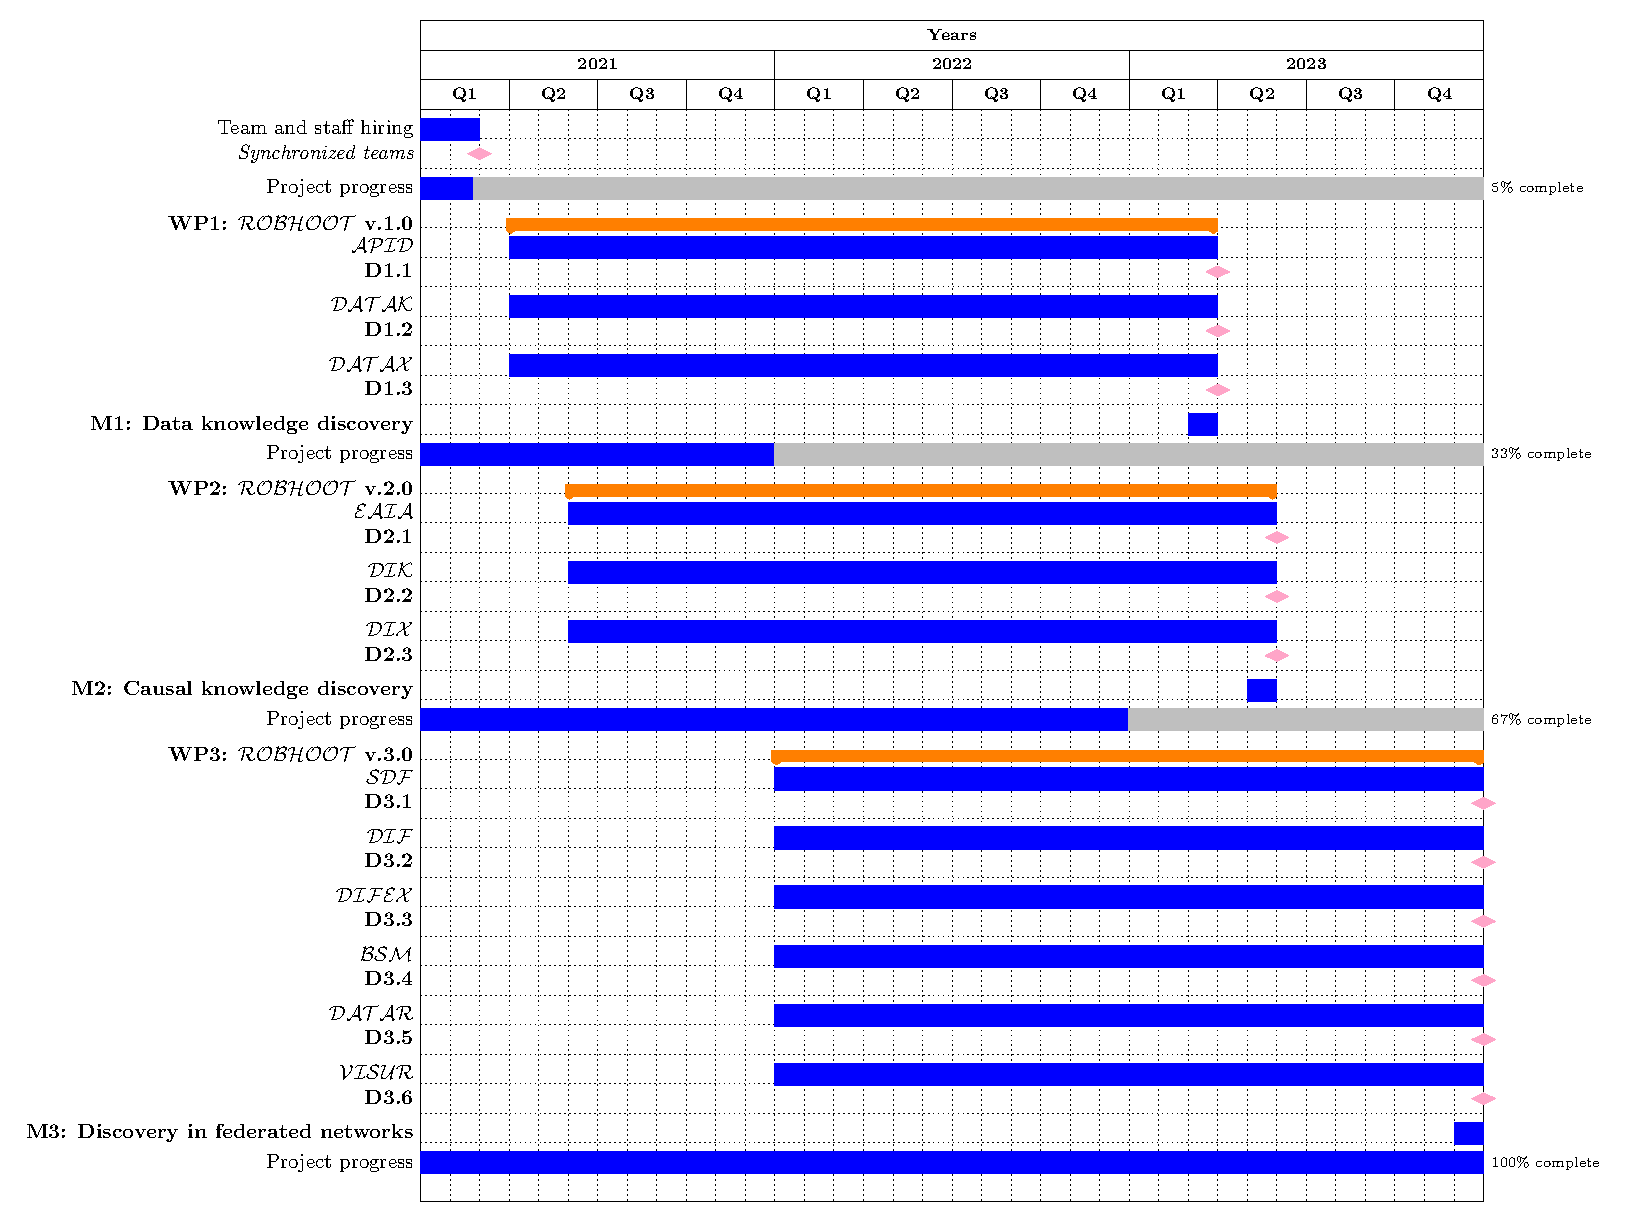
\includegraphics[width=1\textwidth]{Figures/GanttChart.pdf}
   \caption*{{\small {\bf Figure 2: $\mathcal{ROBHOOT}$ Gantt Chart}:
       Work package one, {\bf WP1}, introduces Milestone {\bf
         $\mathcal{ROBHOOT}$ v.1.0} and deliverables one to four ({\bf
         D1.1} to {\bf D1.4}) to bring question- and data-knowledge
       graphs into a global data-architecture map. Work package two,
       {\bf WP2}, introduces Milestone {\bf $\mathcal{ROBHOOT}$ v.2.0}
       and deliverables five to eight ({\bf D2.1} to {\bf D2.4}) to
       fussion automation and interpretable patterns into
       discovery-knowledge graphs. Work package three, {\bf WP3},
       introduces Milestone {\bf $\mathcal{ROBHOOT}$ v.3.0} and
       deliverables nine to eleven ({\bf D3.1} to {\bf D3.3}) to
       connect shared discovery-knowledge graphs to automated
       federated cooperative networks.}}
\end{figure}


\subsubsection{{\bf WP2: $\mathcal{ROBHOOT}$ v.2.0}: \\ Causal-Knowledge Graphs}

  \begin{itemize}
  \item \textcolor{red}{Contrasting explainable biologically inspired
      Causal-Knowledge Graphs for interpretable information when
      dealing with complex sustainability challenges.}
   \item \textcolor{pink}{See Figures 2 and 4}
   \item \textcolor{red}{Contrasting predictions from causal
       open-ended language of models combining Bayesian networks and
       optimization methods}
   \item \textcolor{pink}{See Figures 2 and 4}
   %\item \textcolor{red}{Case study}
   %\item \textcolor{pink}{Covid-19 Causal Knowledge Graph}
   %\item \textcolor{red}{}
   %\item \textcolor{pink}{}
   \end{itemize}

   AI is rapidly advancing in automated discovery (i.e., AutoML
   \citep{Real2020}) making more transparent the processes underlying
   the discovery (i.e., Explainable or interpretable AI
   \citep{Gil2019,Futia2020}). Yet, automated and explainable
   discovery methods are still at an incipient stage of integration,
   particularly in open-ended Bayesian machines
   \citep{Guimera2020}. This is particularly relevant in the context
   of biology, brain research, and evolutionary biology techniques
   where making automatic interpretation of complex systems can
   provide scenarios to help disentangling complex sustainability
   problems for humanity. $\mathcal{ROBHOOT}$ v.2.0 will develop novel
   causal knowledge graphs integrating automated and explainable
   discovery accounting for evolutionary biology and AI techniques
   \citep{Maass2014,Maass2015}. Automatic interpretation of the causal
   processes underlying empirical patterns are explored using
   evolutionary computing and deep learning networks (Table 3.1.1b,
   ({\bf D2.1: Evolutionary Artificial Inteligence Algorithms
     ($\mathcal{EAIA}$)}).

   Evolutionary dynamics explore open-ended language of models
   with varying biologically relevant functions like code insertions,
   deletions, inversions and other molecular and genotype-phenotype
   processes to search for automated biologically inspired solutions
   to complex empirical patterns ({\bf D2.2: Causal-Knowledge Graphs
     ($\mathcal{CKG}$)}, Figure 3a). Causal-knowledge graphs enhances
   the connection between automated and explainable AI throughout
   prediction and knowledge power (Figure 3b). Automated and
   interpretable data inference still present many challenges in the
   context of multidimensional landscapes
   \citep{OHare2015,Cranmer2019}. This is particularly relevant in
   Earth and Ecosystem science and Biodiversity and Sustainability
   science \citep{Reichstein}, where merging automation to
   interpretable data might increase human ability to make stronger
   inferences about future sustainability challenges and solutions. In
   order to make inference from complex data more robust we contrast
   predictions from Evolutionary Neural Networks in the framework of
   Bayesian Space Models to explore open-ended language of models
   combining Bayesian networks and optimization methods ({\bf D2.3:
     Bayesian Space Models ($\mathcal{BSM}$)}. The Bayesian space
   models module ensures the search, the evaluation of models,
   trading-off complexity, fitting to the data and quantify resource
   usage \citep{Guimera2020,Steinruecken}. $\mathcal{ROBHOOT}$ v.2.0
   deploys the COVID-19 pandemic as a case study to automatically
   infer interpretable causal-knowledge graphs at global scale ({\bf
     D2.4: COVID-19 Causal-Knowledge Graphs ($\mathcal{COCAU}$)}).

 \begin{figure}[h!]
   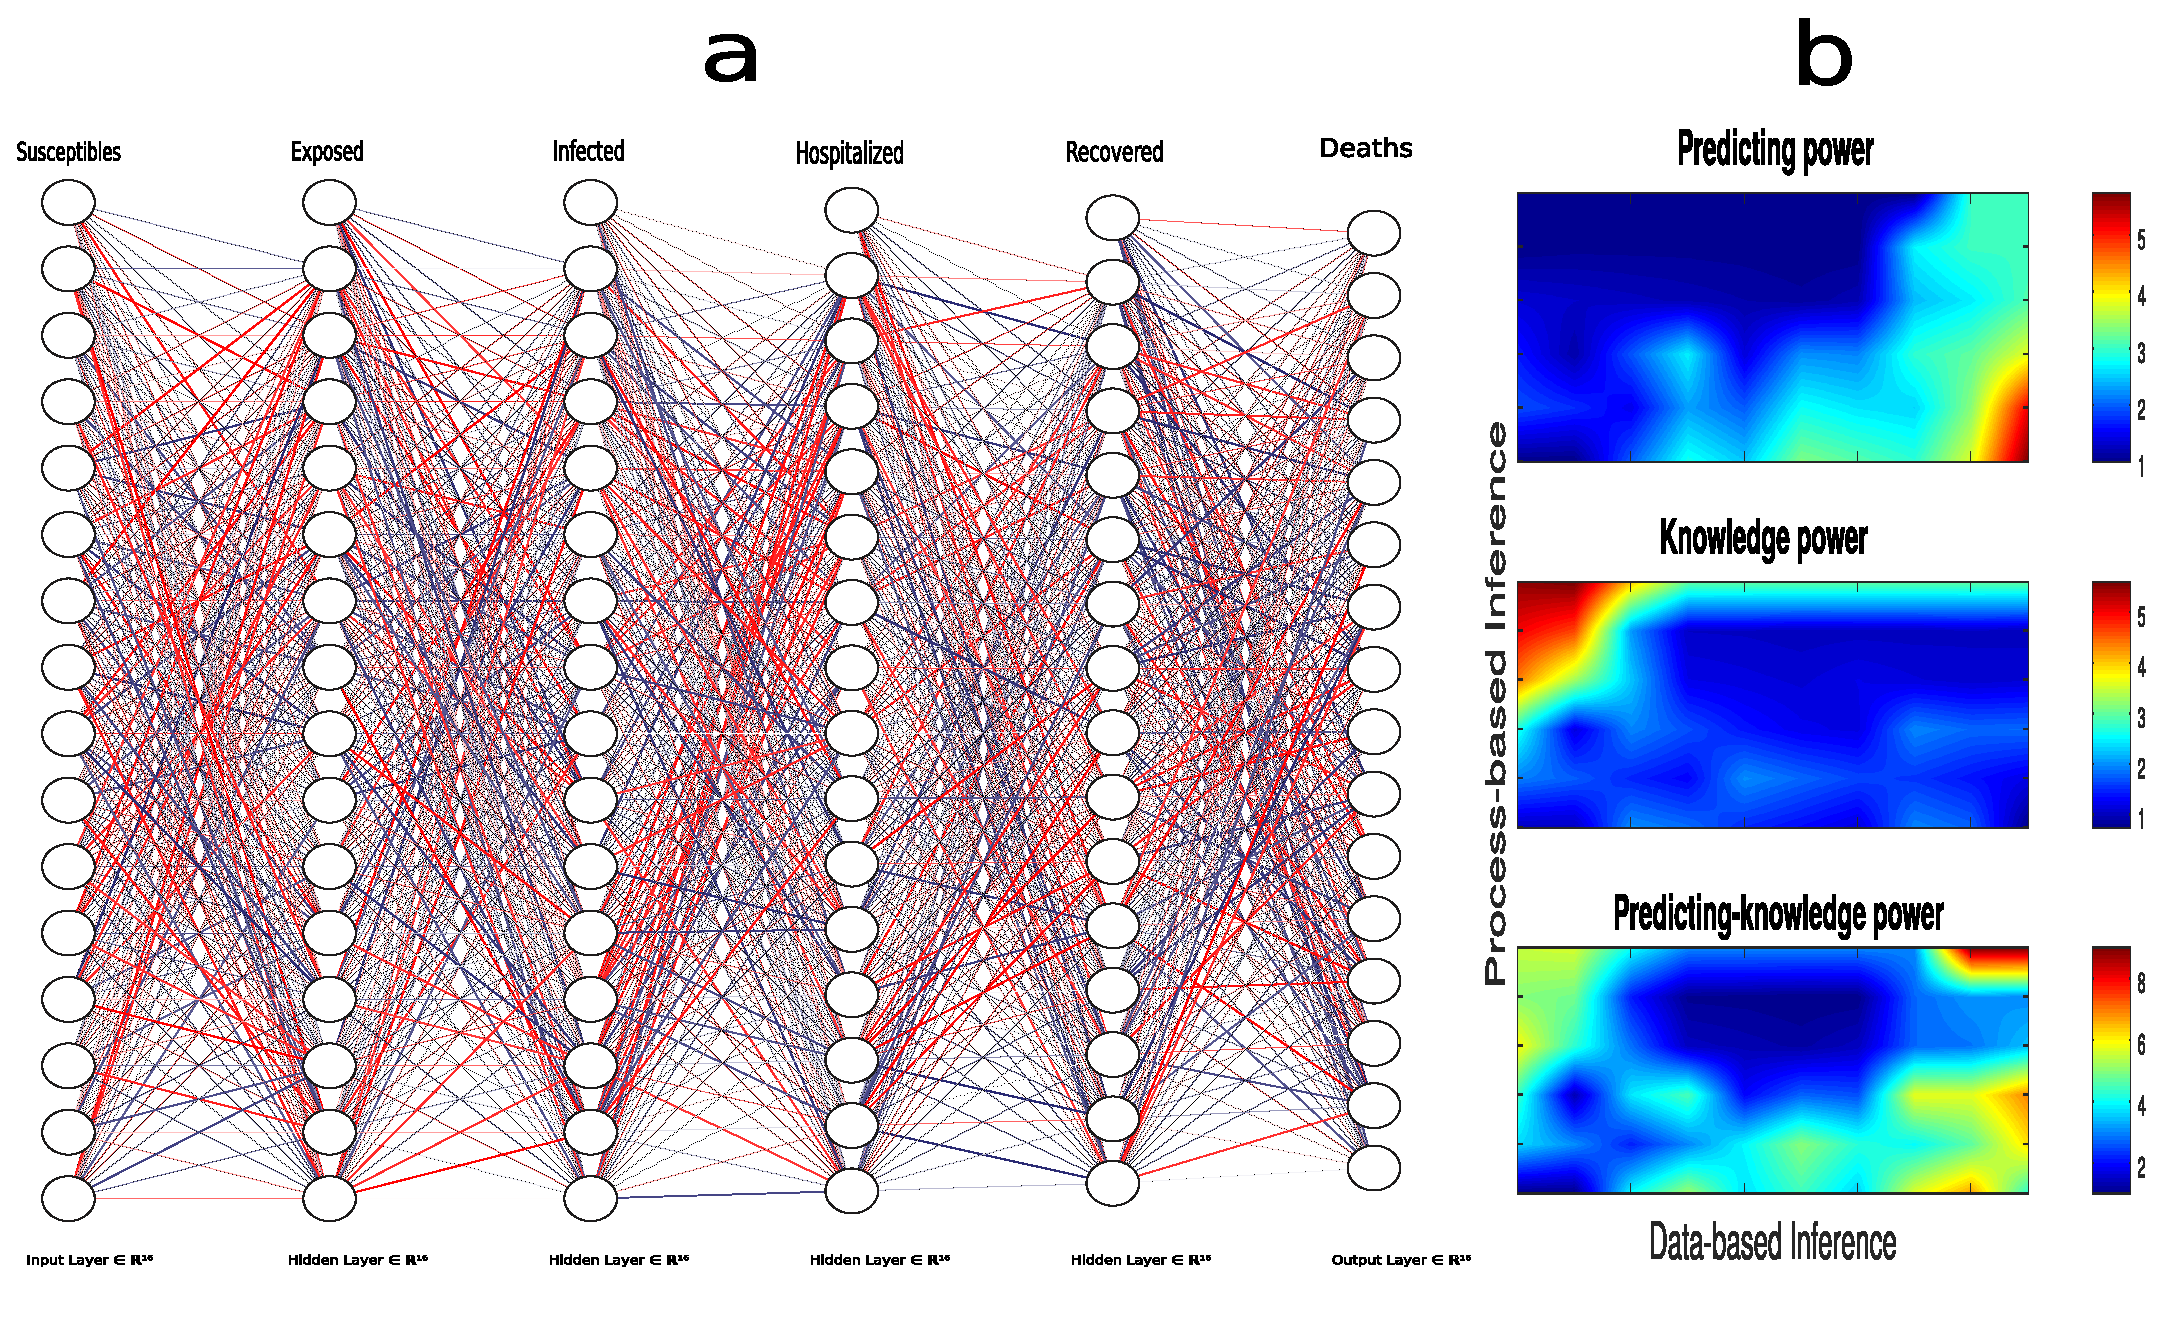
\includegraphics[width=1\textwidth]{Figures/Figure3integrated.pdf}
   {\small {\bf Figure 3: Causal-Knowledge Graphs}. {\bf a}) They
     contain features of deep learning networks and process-based
     modeling making empirical patterns interpretable. For
     epidemiology models, for example, all input, hidden and output
     layers (bottom) can be ``converted'' to age-class susceptibles
     (input), exposed, infected, hospitalized, and recovered (all
     hidden), and deaths (output). The same applies to edges
     connecting each pair of nodes. Causal-Knowledge Graph recovers
     the temporal sequence of events that best predict the output
     layer (i.e., Deaths). {\bf b)} Causal-Knowledge Graphs integrates
     predicting and knowledge power into interpretable knowledge
     (bottom, b). x-axis represents ``Data-based inference'' (i.e.,
     gradient of AI methods from low (left) to high (right) predicting
     power). y-axis represents ``Process-based inference'' (i.e.,
     gradient of process-based methods from low (bottom left) to high
     (top left) knowledge power). The gradient of predicting power map
     (top) shows a hot spot red area in the bottom right highlighting
     the region where AI methods best predict the empirical data. The
     gradient of knowledge power map (middle) shows a red hot spot in
     the top left highlighting the region where the best mechanistic
     understanding occur. The predicting-knowledge power map (bottom)
     shows the sum of the two previous maps highlighting a red hot
     spot where predicting and knowledge power occur. Red and blue
     lines show important and non-important roles in the
     predicting-knowledge power map, respectively.}
\end{figure}


%Deliverable table  
\begin{table}[h!]
\begin{center}
  \begin{tabular}{|m{2cm} || m{1.25cm} || m{1.75cm} || m{1.55cm} || m{2.4cm} || m{1.7cm} || m{1.15cm} || m{1.7cm}|}
  \hline\hline
  \rowcolor{lightpink!30}
  {\bf $\mathcal{ROBHOOT}$ v.X.X} & {\bf Deliver. number} & {\bf Deliver. name} & {\bf WP} & {\bf Name Lead} & {\bf Type} & {\bf Disem.} & {\bf Delivery date} \\
  \hline\hline
  \rowcolor{piggypink!20}
  {\bf v.1.0} & {\bf D1.1} & $\mathcal{APID}$ & WP1 & {\bf Fortuna} & OT & PU & 27 \\
  \hline\hline
  \rowcolor{piggypink!20}
  {\bf v.1.0} & {\bf D1.2} & $\mathcal{QKG}$ & WP1 & {\bf Egu\'iluz} & OT & PU  & 27 \\
  \hline\hline
   \rowcolor{piggypink!20}
  {\bf v.1.0} & {\bf D1.3} & $\mathcal{DKG}$ & WP1 & {\bf Choirat} & OT & PU  & 27 \\
  \hline\hline
  \rowcolor{piggypink!20}
  {\bf v.1.0} & {\bf D1.4} & $\mathcal{CODA}$ & WP1 & {\bf Leads M1} & R,OT,DEC & PU  & 28 \\
    \hline\hline
 \rowcolor{piggypink!40}
  {\bf v.2.0} & {\bf D2.1} & $\mathcal{EAIA}$ & WP2 & {\bf Meli\'an} & OT & PU & 29 \\
  \hline\hline
  \rowcolor{piggypink!40}
  {\bf v.2.0} & {\bf D2.2} & $\mathcal{CKG}$ & WP2 & {\bf Baity/Vicente} & OT & PU  & 29 \\
  \hline\hline
   \rowcolor{piggypink!40}
  {\bf v.2.0} & {\bf D2.3} & $\mathcal{BSM}$ & WP2 & {\bf Guimer\`a} & OT & PU  & 29 \\
  \hline\hline
  \rowcolor{piggypink!40}
    {\bf v.2.0} & {\bf D2.4} & $\mathcal{COCAU}$ & WP2 & {\bf Leads M2} & R,OT,DEC & PU & 30 \\
    \hline\hline
 %   \rowcolor{piggypink!60}
  %{\bf v.3.0} & {\bf D3.1} & $\mathcal{SDN}$ & WP3 & NAME LEAD & OT & PU  & 29 \\
  %\hline\hline
 % \rowcolor{piggypink!60}
 % {\bf v.3.0} & {\bf D3.2} & $\mathcal{SCN}$ & WP3 & NAME LEAD & OT & PU & 30 \\
 % \hline\hline
   \rowcolor{piggypink!60}
  {\bf v.3.0} & {\bf D3.1} & $\mathcal{SDN}$ & WP3 & {\bf von Waldow} & OT & PU & 42 \\
  \hline\hline
  %\rowcolor{piggypink!60}
  %{\bf v.3.0} & {\bf D3.4} & $\mathcal{CODIN}$ & WP3 & von Waldow & R,OT,DEC & PU & 32 \\
  % \hline\hline
  %\rowcolor{piggypink!80}
  %{\bf v.4.0} & {\bf D3.2} & ADAN & WP4 & NAME LEAD & OT & PU & 35 \\
  %\hline\hline
  %\rowcolor{piggypink!80}
  %{\bf v.4.0} & {\bf D4.2} & ACAN & WP4 & NAME LEAD & OT & PU & 36 \\
  %\hline\hline
   \rowcolor{piggypink!80}
  {\bf v.3.0} & {\bf D3.2} & $\mathcal{ADIN}$ & WP3 & {\bf Maass} & OT & PU & 42 \\
  \hline\hline
  \rowcolor{piggypink!80}
  {\bf v.3.0} & {\bf D3.3} & $\mathcal{ACODIN}$ & WP3 & {\bf Leads M1-3} & R,OT,DEC & PU & 42 \\
\hline\hline
  \end{tabular}
\end{center}
\caption*{{{\bf Table 3.1c List of Deliverables}: {\bf $\mathcal{ROBHOOT}$}
    contains three main work packages: Milestone {\bf
      $\mathcal{ROBHOOT}$ v.1.0} span from Month 3 to 27. Deliverable
    {\bf D1.4 ($\mathcal{CODA}$)}, the global COVID-19
    data-architecture depends on all the deliverables of work package
    one ({\bf WP1}). Milestone {\bf $\mathcal{ROBHOOT}$ v.2.0} span
    from Month 5 to 29. Deliverable {\bf D2.4 ($\mathcal{COCAU}$)},
    interpretable causal-knowledge graph for COVID-19 depends on all
    the deliverables of work package two ({\bf WP2}), and Milestone
    {\bf $\mathcal{ROBHOOT}$ v.3.0} span from Month 18 to
    42. Deliverable {\bf D3.3 (ACODIN)}, automated cooperative
    forecasting of discovery-knowledge graph for the COVID-19 depends
    on all the deliverables of work package three ({\bf WP3}).}}
\end{table}

 
\subsubsection{{\bf WP3: $\mathcal{ROBHOOT}$ v.3.0}: \\ Automated
  Discovery-Knowledge Graphs in Federated Networks}

   \begin{itemize}
   \item \textcolor{red}{A science-based explainable-knowledge graph
       technology is not enough if we aim to globally contrast
       robustly paths for interpretation of causal process predicting
       global data-architectures.}
   \item \textcolor{pink}{A science-based technology to develop shared
       cooperative forecasting in federated networks in face of
       rapidly emerging global emergency and sustainability
       challenges.}
  \item \textcolor{red}{Science-based explainable discovery-knowledge
      graphs shared in a federated network is not enough if most
      contributions can not be reproduced and strongly depend on
      competitive schemes. This might be particularly relevant in the
      face of rapidly responding to global emergency and
      sustainability challenges.}
  \end{itemize}

  A science-based explainable technology is not enough if we aim to
  globally contrast robustly interpretable causal processes predicting
  the global data-architecture obtained from merging data- and
  causal-knowledge graphs. Similarly, science-based explainable
  discovery-knowledge graphs shared in a federated network are not
  enough if most contributions can not be reproduced and strongly
  depend on competitive schemes. In this regard, federated objects can
  be seen as networks containing many types of nodes (i.e., like a
  diversity of neurons) with varying connectivity and firing
  probabilities \citep{Maass2014,Maass2015} sharing causal-knowledge
  graphs according to given rules to find populations of
  causal-knowledge graphs that best fit to the data-knowledge graphs
  patterns. Sharing data- and causal-knowledge graphs need novel
  (firing, spiking... etc) protocols to enhance forecasting and strong
  inference in federated networks. $\mathcal{ROBHOOT}$ v.3.0 develops
  protocols in digital networks to embed explainable
  discovery-knowledge graphs into global cooperation schemes to
  increase robustness and reproducibility of discovery-knowledge graphs
  \citep{Dilley2016}. Technologies in decentralized digital ecosystems
  are rapidly advancing in a variety of sectors. Most progress is
  coming from the scalability, security and decentralization fronts
  \citep{Golem2016,Dilley2016,Durov2017,Androulaki2018,OceanProtocolFoundation2018,BigchainDBGmbH2018}. In
  the science ecosystem, only a few applications of open decentralized
  technologies exist \citep{Gunther2018}. Yet, sharing reproducible
  data- and causal-knowledge graphs, the discovery-knowledge graphs,
  along cooperative networks to facilitate forecasting is currently
  not in place.

  This is particularly relevant in the face of rapidly responding to
  global emergency and sustainability challenges. For example, in the
  context of the COVID-19 pandemic, and in many other situations
  challenging global sustainability, models and predictions abound,
  but no one can say with certainty what the course of the virus or
  the focus of the causing factors will be, and much less the impact
  the pandemic will have on people and societies
  \citep{Deloitte2020}. In such an scenario, sharing fully
  reproducible contributions from a large number of nodes following
  standard protocols containing discovery-knowledge graphs can guide
  us to improve the robustness of the forecasting.
  
  $\mathcal{ROBHOOT}$ v.3.0} deploys sharing protocols of
discovery-knowledge graphs using reproducible-knowledge graphs, {\bf
  D3.1, Sharing discovery-knowledge graphs in federated networks
  ($\mathcal{SDN}$)}. This deliverable explores scalability and
security properties of sharing discovery-knowledge graphs using
different topologies of federated networks: there can be data-, and
causal-knowledge graphs belonging to specific categories and they
might be integrated with different data- and causal-types to gain
global understanding of data and interpretable patterns (i.e., like
letting people on different social networks follow each
other). Second, $\mathcal{ROBHOOT}$ v.3.0 connects interpretable
discovery-knowledge graphs to fedetated netwoks to study the
properties of automated cooperative forecasting and strong inference
in the face of global sustainability challenges ({\bf D3.2, Automated
  discovery in federated networks ($\mathcal{ADIN}$)}).

%Despite the dramatic rise in global pandemics during the last decade
%(i.e., the SARS pandemic in 2003, to Avian Influenza in 2006, H1N1 in
%2009, Ebola in 2014, the appearance of the Zika virus in Latin America
%in 2015, and the current Covid-19 pandemic), with these developments
%inextricably bound up in modern socio-technical developments and
%processes of globalization, science-based technologies facilitating
%rapid sharing of information to mitigate risks and enhance global
%cooperative forecasting to efficiently respond with informed scenarios
%are particularly lacking \citep{Wilson2018}. The last deliverable of
%$\mathcal{ROBHOOT}$ v.3.0, {\bf D3.3: Automated Cooperative
%  Forecasting of Discovery-Knowledge Graphs for the COVID-19 case
%  study ($\mathcal{ACODIN}$)}, deploys automated discovery-knowledge
%graphs in federated networks for the COVID-19 case study to contrast
%cooperative forecasting scenarios at a global scale.

\begin{comment}
\begin{table*}[ht]
 %\rowcolor{pink}
\begin{tabular}{ p{3.5cm} | p{14cm}}
  \hline \hline
  \textbf{Feature} &\textbf{$\mathcal{ROBHOOT}$}\\  \hline
  Long-term vision & Global open-access to a fully reproducible knowledge-generation inspired technology \\ \hline
  Breakthrough scientific and technological target & Collapsing evidence- and research-based knowledge gaps for a sustainable knowledge-inspired society\\ \hline
  Novelty & Science-based technology emerging from targeted algorithmic discovery at the interface of multilayer networks, knowledge graphs, deep-learning, and consensus mechanisms\\ \hline
  Foundational & Neutral-knowledge inspired technology for an emerging open science of science and science-society research disciplines \\ \hline
  High-risk & Adapted to explore new terrirories into the open-science-technology-society interface ecosystem \\ \hline
  Interdisciplinarity & Hybridizing expertise from distributed computing and deep learning to multilayer networks and the ecology and evolution of natural and digital ecosystems (Table 1) \\ \hline
  \bottomrule

\end{tabular}
\caption{{\bf $\mathcal{ROBHOOT}$} features along its developmental stages.}
\end{table*}
\end{comment} 



  \begin{comment}
    %\centering
  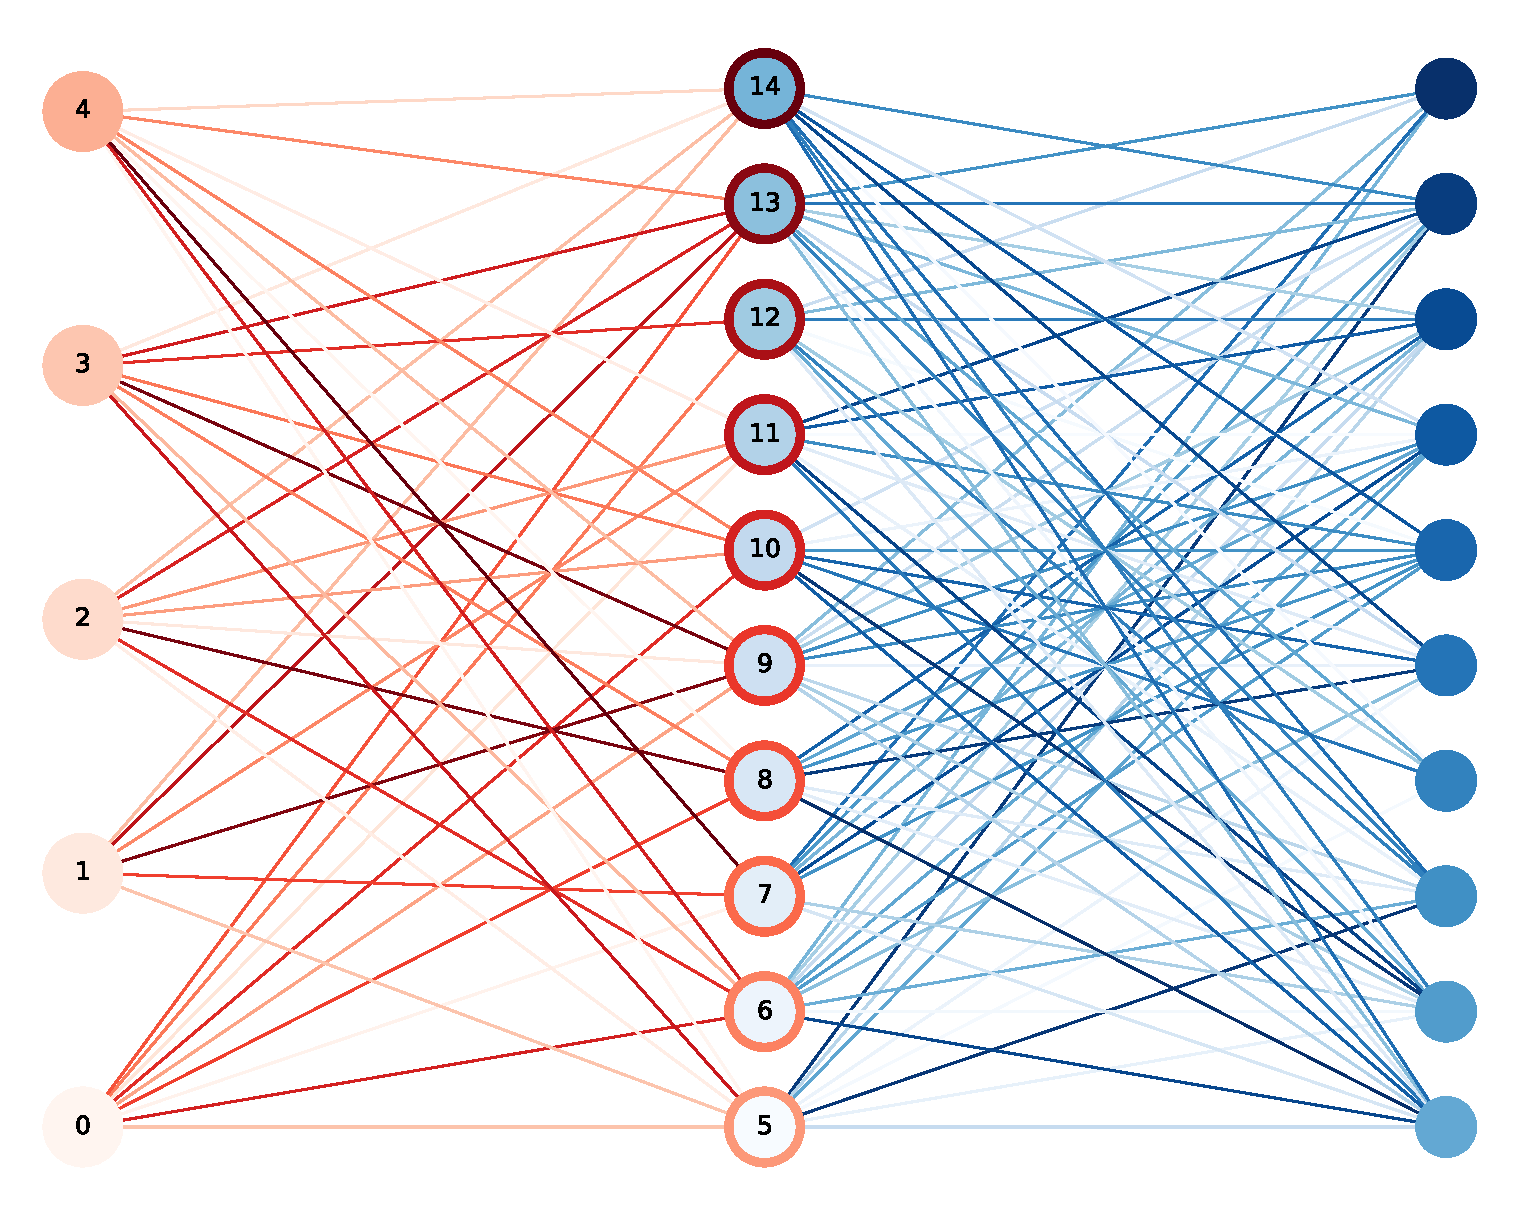
\includegraphics[width=0.45\textwidth]{Figures/FigureRobhoot.pdf}
 
  {\small {\bf Figure 3: Robhoot in Digital Ecosystems}: {\bf Left
      column}: {\bf $\mathcal{ROBHOOT}$ v.1.0} representing the
    research cycle as nodes from number 0 to 4: Data integration (0),
    Complexity Reduction (1), Inference (2), Validation (3), and
    Visualization(4)). {\bf Central column}: Nodes representing the
    research cycle in the left column are connected to open-source
    software in the digital ecosystem. Connections with node number 0
    in the left column can, for example, represent the ETLs
    open-source software interactions required to generate the {\bf
      Universal ETLs} module. The same meaning applies to the
    different nodes of the left column. {\bf Right column}: Each node
    represents a report meaning there is a reporting gradient
    generated by the connections to the open-source software from
    where each report is generated only using a subset of the research
    layers and open-source software.}
\end{comment}


\subsection{Management structure, milestones and procedures}

\begin{itemize}
  \item \textcolor{red}{Describe the organisational structure and the
      decision-making (including a list of milestones (table 3.2a))}
\item \textcolor{red}{Explain why the organisational structure and
  decision-making mechanisms are appropriate to the complexity and
  scale of the project.}
\item \textcolor{red}{Describe any critical risks, relating to project
    implementation, that the stated project's objectives may not be
    achieved. Detail any risk mitigation measures. Please provide a
    table with critical risks identified and mitigating actions (table
    3.2b) and relate these to the milestones.}
\end{itemize}

Advisory board covering the weakest parts of the proposal -- mention here



%Milestone table  
\begin{table}[h!]
\begin{center}
  \begin{tabular}{|m{1.75cm} || m{2.5cm} || m{2.5cm} || m{2.4cm} || m{6cm}|}
   \hline\hline
   \hline\hline
  \rowcolor{lightpink!30}
  {\bf Milestone number} & {\bf Milestone name} & {\bf Related work package(s)} & {\bf Due data (months)} & {\bf Verification} \\
  \hline\hline
  \rowcolor{piggypink!20}
  {\bf M1} & {\bf Discovery-Knowledge Graph}  & WP1-WP2 & 27 & OS-Software,Paper/Conf. &
  \hline\hline
  \rowcolor{piggypink!40}
  {\bf M2} & {\bf Evolutionary Automation} & WP2 & 29 & OS-Software,Paper/Conf.,demo-website &
  \hline\hline
   \rowcolor{piggypink!60}
  {\bf M3} & {\bf Cooperative Forecasting} & WP3 & 42 & OS-Software,Paper/Conf.,main-website &
  \hline\hline
  %\rowcolor{piggypink!80}
  %\bf M4} & {\bf $\mathcal{ROBHOOT}$ v.4.0} & WP4 & Months 21-42 & OS-Software,Paper/Conf.,official website &
  %\hline\hline
\hline\hline
  \end{tabular}
\end{center}
\caption*{{{\bf Table 3.2a: List of Milestones}: {\bf $\mathcal{ROBHOOT}$} contains
    three milestones: {\bf $\mathcal{ROBHOOT}$ v.1.0} span from Month
    3 to 27 to generate open-source software and research papers
    and/or conferences for the Data-Knowledge Graph. {\bf
      $\mathcal{ROBHOOT}$ v.2.0} span from Month 5 to 29 producing the
    the integration between the Data-, and the Causal-Knowledge Graph,
    the Discovery-Knowledge Graph, as a open-source software and
    research papers and/or conferences and public demo-website. {\bf
      $\mathcal{ROBHOOT}$ v.3.0} span from Month 18 to 42 to build a
    prototype of Discovery-Knowledge Graphs in Federated Cooperative
    Networks as an official {\bf $\mathcal{ROBHOOT}$} website.}}
\end{table}

  \subsection{Consortium as a whole}

  \begin{itemize}
  \item \textcolor{red}{The individual members of the consortium are
      described in a separate section 4}
    \item \textcolor{red}{Describe the consortium. Explain how it will
        support achieving the project objectives.  Does the consortium
        provide all the necessary expertise? Is the
        interdisciplinarity in the breakthrough idea reflected in the
        expertise of the consortium?}
    \item \textcolor{red}{In what way does each of the partners
        contribute to the project? Show that each has a valid role and
        adequate resources in the project to fulfil that role. How do
        the members complement one another? Other countries and
        international organisations: If one or more of the
        participants requesting EU funding is based in a country or is
        an international organisation that is not automatically
        eligible for such funding (entities from Member States of the
        EU, from Associated Countries and from one of the countries in
        the exhaustive list included in General Annex A of the work
        programme are automatically eligible for EU funding), explain
        why the participation of the entity in question is considered
        essential for carrying out the action on the grounds that
        participation by the applicant has clear benefits for the
        consortium.}
  \end{itemize}

  {\bf $\mathcal{ROBHOOT}$} is a science-enabled multi-feature
  technology. $\mathcal{ROBHOOT}$'s consortium is designed with a
  highly modular topology to gain functionality within each milestone
  (Figure 4, blue, red, and pink). From the other side, connections
  among the modules reflect the emergence of interdisciplinarity
  technologies, the Discovery-Knowledge Graph, The Evolutionary
  Automation and the Cooperative Forecasting (Figure 4, green). {\bf
    $\mathcal{ROBHOOT}$ v.1.0}'s team is composed by Fortuna,
  Egu\'iluz and Choirat to bring question- and data-knowledge graphs,
  the data-discovery process, to fully reproducible-knowledge graphs
  (section 3.1 and Figure 4). Milestone one requires a mixture of
  researchers: computer-, data-scientists and developers and
  researchers working in complex networks from the quantitative and
  epistemological angles. Fortuna's, Egu\'iluz and Choirat's expertise
  complement each other's roles: Fortuna's team takes care of
  Data-Knowledge Graphs following ontology standards and automated
  API-Discovery (i.e., {\bf $\mathcal{APID}$} and {\bf
    $\mathcal{QKG}$, $\mathcal{DKG}$}). Egu\'iluz's team focuses on
  network modularity, community detection and decentralization
  metrics, to characterize Question-, and Data-Knowledge Graphs (i.e.,
  {\bf $\mathcal{QKG}$} and {\bf $\mathcal{DKG}$}, and Choirat's team
  encodes all the algorithms and procedures from Fortuna's and
  Egu\'iluz's teams into Reproducible-Knowledge Graphs. Milestone {\bf
    $\mathcal{ROBHOOT}$ v.1.0} generates an automated COVID-19
  Data-Knowledge Graph (Figure 4, blue).

  {\bf $\mathcal{ROBHOOT}$ v.2.0}'s team composed by Guimer\`a, Baity,
  Vicente, and Meli\'an fussion Bayesian Machine Scientist to
  Evolutionary and AI Algorithms, the Evolutionary Automation (Figure
  4, green), making interpretable data patterns along causal-knowledge
  graphs. The team for this milestone add complementarity expertise to
  {\bf $\mathcal{ROBHOOT}$ v.1.0}'s team: Now the skills focus on
  data-scientists trained in deep learning networks and automation
  algorithms, theoreticians with expertise in Bayesian inference, and
  evolutionary biologists with expertise in empirical patterns and
  evolutionary-inspired networks (section 3.2 and Figure 4,
  red). Despite modules {\bf $\mathcal{ROBHOOT}$ v.1.0} and {\bf
    $\mathcal{ROBHOOT}$ v.2.0} focus on specific milestones and
  deliverables (Figure 2 and 4), they have functional interactions
  because data- and causal-knowledge graphs, the discovery-knowledge
  graphs, will be fussioned using evolutionary automation built on a
  interdisciplinarity science-enabled technology that can be compactly
  converted into user-friendy open-software ({\bf Discovery-Knowledge
    Graphs} and {\bf Evolutionary Automation}, green). Milestone {\bf
    $\mathcal{ROBHOOT}$ v.2.0} generates an automated COVID-19
  Causal-Knowledge Graph (Figure 4, red). Thus, interdisciplinarity
  enters not only at the intra-module development stage, but also at
  the inter-module stage where discovery-knowledge graphs and
  evolutionary automation form the basis for a interdisciplinarity
  breakthrough reflected in the highly complementarity skills of the
  consortium (section 4.1). The first two modules in {\bf
    $\mathcal{ROBHOOT}$} contain researchers from Estonia, Spain,
  Switzerland and Sweden ({\bf Computer software design, To be
    confirmed}).
  
  The {\bf $\mathcal{ROBHOOT}$} consortium wants to advance the
  rapidly evolving digital ecosystem by making cooperative discovery a
  fundamental feature of it. For this purpose, a science-based
  automated and interpretable technology is not enough if we aim to
  contrast robustly interpretable scenarios in the face of global
  sustainability challenges. To achieve scalability for the
  discovery-knowledge graphs, sharing and automation in federated
  cooperation networks is the excellency feature of {\bf
    $\mathcal{ROBHOOT}$ v.3.0} (section 3.3). {\bf $\mathcal{ROBHOOT}$
    v.3.0}'s team composed by von Waldow and Maass, develops protocols
  for sharing the discovery-knowledge graphs along federated
  networks. The team forming {\bf $\mathcal{ROBHOOT}$ v.3.0} therefore
  requires quite a lot of contrasting skills. First, developers
  working in P2P and security protocols. Second, social scientists
  computer scientists and neurobiologists in collaboration to
  developers aiming to build user-friendly open-access interfaces to
  explore scenarios of automated reproducible sharing in federated
  networks. Milestone {\bf $\mathcal{ROBHOOT}$ v.3.0} is a fundamental
  stepping-stone for developing cooperative forecasting: it first
  guarantees discovery-knowledge graphs are reproducible shareable
  objects. Yet, in the same way than evolutionary algorithms and the
  Bayesian machine scientist search automatically for open-ended space
  models to generate the most plausible causal-knowledge graphs, the
  discovery-knowledge graphs produced in different nodes need to
  automatically interact and learn from each other to find better
  forecasting scenarios at a global scale. $\mathcal{ROBHOOT}$
  v.3.0}'s implements the cooperation and automation among
discovery-knowledge graphs in federated networks for making
cooperative forecasting a standard global property. Milestone {\bf
  $\mathcal{ROBHOOT}$ v.3.0} generates an Automated COVID-19 DKGs in
Federated Cooperation Networks (Figure 4, pink). $\mathcal{ROBHOOT}$
v.3.0} contain researchers from Switzerland and Austria.

\begin{figure}[h!]
  \floatbox[{\capbeside\thisfloatsetup{capbesideposition={right,top},capbesidewidth=4cm}}]{figure}[\FBwidth]
  {\caption*{Figure 4: $\mathcal{ROBHOOT}$ Consortium: {\bf
        $\mathcal{ROBHOOT}$ v.1.0} (blue) to {\bf $\mathcal{ROBHOOT}$
        v.3.0} (pink) with acronyms of each deliverable (Left column),
      tasks (Center), and lead name (Right column). Links connect
      deliverables to tasks and leading groups. $\mathcal{ROBHOOT}$
      delivers three interdisciplinarity-driven science-enabled
      technologies: {\bf Discovery-Knowledge Graph} connecting {\bf
        $\mathcal{ROBHOOT}$ v.1.0} and {\bf $\mathcal{ROBHOOT}$
        v.2.0}. {\bf Evolutionary automation} in {\bf
        $\mathcal{ROBHOOT}$ v.2.0}, and {\bf Cooperative forecasting}
      connecting {\bf $\mathcal{ROBHOOT}$ v.2.0} to {\bf
        v.3.0}}}
    %\label{fig:test}
  {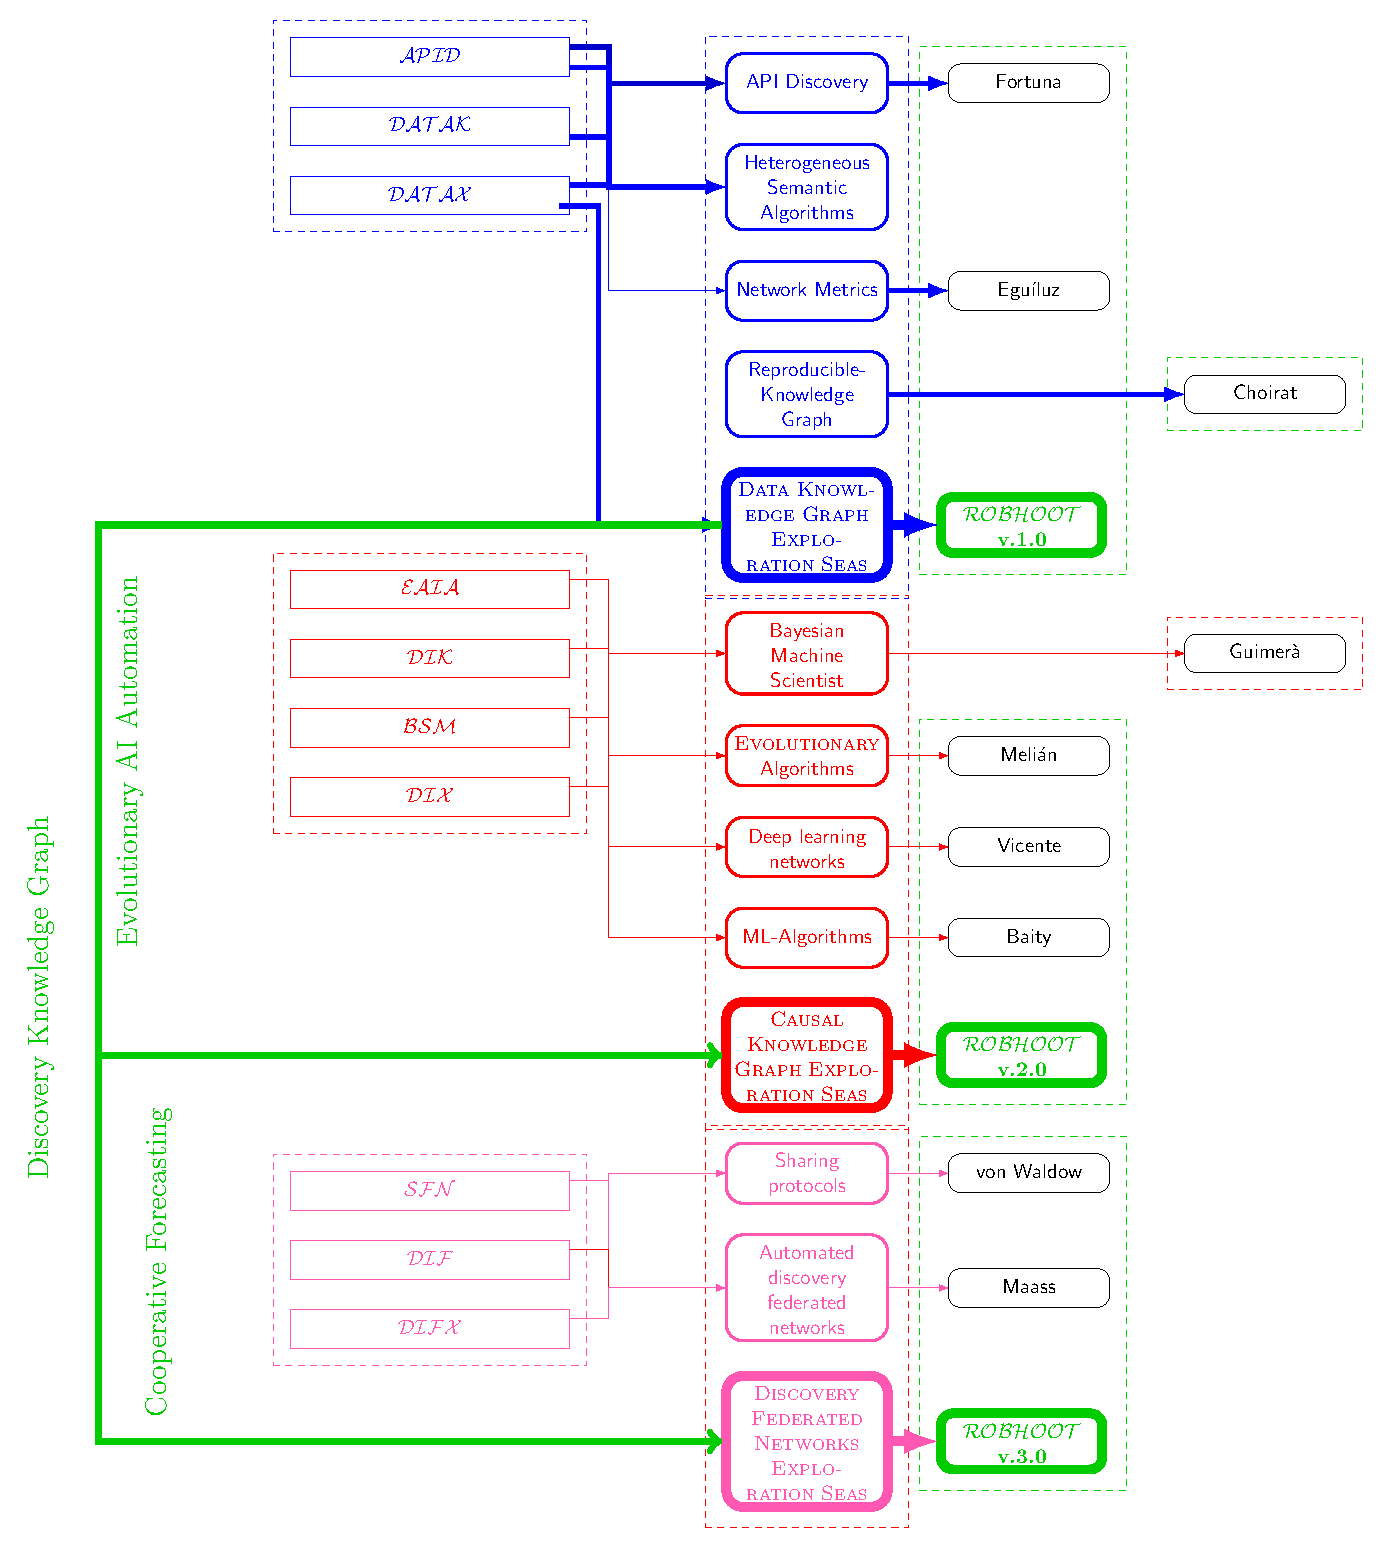
\includegraphics[width=9.75cm,height=22cm]{Figures/Consortium.pdf}}
\end{figure}
  
  
  \subsection{Resources to be committed}
 
  \begin{itemize}
  \item \textcolor{red}{Please make sure the information in this
      section matches the costs as stated in the budget table in
      section 3 of the administrative proposal forms, and the number
      of person months, shown in the detailed work package
      descriptions.  Please provide the following:}
 \item \textcolor{red}{a table showing number of person months required
    (table 3.4a)}
  \item \textcolor{red}{a table showing ‘other direct costs’ (table
      3.4b) for participants where those costs exceed 15\% of the
      personnel costs (according to the budget table in section 3 of
      the administrative proposal forms)}
\end{itemize}

  

\newpage

\section{Members of the consortium}

\begin{comment}
 This section is not covered by the page limit.

 The information provided here will be used to judge the operational
 capacity. Please make sure that you do not include information here
 that relates to the headings under sections 1 to 3. Experts will be
 instructed to ignore any information here which appears to have been
 included to circumvent page limits applying to those sections.
 \end{comment}

 \subsection{Participants (applicants)}

 \begin{itemize}
 \item \textcolor{red}{For each participant, provide the following: a
     description of the legal entity and its main tasks, with an
     explanation of how its profile matches the tasks in the proposal}
 \item \textcolor{red}{a curriculum vitae or description of the
     profile of the persons, including their gender, who will be
     primarily responsible for carrying out the proposed research
     and/or innovation activities. Indicate each person who would be a
     first-time participant to FET under Horizon 2020}
\item \textcolor{red}{a list of up to 5 relevant publications, and/or
    products, services (including widely-used datasets or software),
    or other achievements relevant to the call content}
\item \textcolor{red}{List of up to 5 relevant previous projects or
    activities, connected to the subject of this proposal}
 \item \textcolor{red}{a description of any significant infrastructure
     and/or any major items of technical equipment, relevant to the
     proposed work}
 \item \textcolor{red}{if operational capacity cannot be demonstrated
     at the time of submitting the proposal, describe the concrete
     measures that will be taken to obtain it by the time of the
     implementation of the task}
 \end{itemize}


 \begin{itemize}
 \item (description legal identity) Dr. Carlos Meli\'an is a tenured
   researcher in Theoretical Evolutionary Ecology at EAWAG, ETH-Domain
   in Switzerland, and associate professor at the University of Bern.
       (CV, gender, responsible research proposed, first time participant FET)

       He is the principal coordinator of the proposal.  Dr. Meli\'an
       has broad expertise in evolutionary algorithms and
       eco-evolutionary dynamics in ecological communities and
       biodiversity.
  
       (5 pubs)
       • Melián C, et al. 2018. Deciphering the interdependence
       between ecological and evolutionary networks. Trends in ecology
       & evolution 33,7: 504-512.  • Andreazzi C, Guimaraes P, Melián
       C. 2018. Eco-evolutionary feedbacks promote fluctuating
       selection and long-term stability of antagonistic
       networks. Proc. R. Soc. B 285: 20172596.  • Melián C, Seehausen
       O, Eguiluz V, Fortuna M, Deiner K. 2015. Diversification and
       Biodiversity Dynamics of Hot and Cold Spots. Ecography 38,
       393-401.  • Melián C, et al. 2015. Dispersal dynamics in food
       webs. American Naturalist 185, 2: 157-168.  • Melián C., et
       al. 2014. Individual trait variation and diversity in food
       webs. Advances in Ecological Research. Vol. 50. Academic Press,
       207-241.



 \item {\bf Victor M. Egu\'iluz (IFISC, CSIC, Spain)}: IFISC is an
   Maria de Maetzu Excellent center at the UIB, Balearic
   Islands. Dr. Egu\'iluz has expertise in health-related topics, in
   particular he has developed collaborations with Harvard medical
   school and many biodiversity and sustainability research
   institutions. The group of the PL has worked in the development of
   data-driven agent-based networks in social, biological and
   environmental problems with particular relevance in epidemiological
   networks.
\item
\item
   \end{itemize}

 
 \subsection{Third parties involved in the project (including use of third party resources)}


\begin{itemize}
\item \textcolor{red}{For each participant, does the participant plan
    to subcontract certain tasks (please note that core tasks of the
    project should not be sub-contracted) Y/N If yes, please describe
    and justify the tasks to be subcontracted}
\item \textcolor{red}{Does the participant envisage that part of its
    work is performed by linked third parties2 Y/N If yes, please
    describe the third party, the link of the participant to the third
    party, and describe and justify the foreseen tasks to be performed
    by the third party}
\item \textcolor{red}{Does the participant envisage the use of
    contributions in kind provided by third parties (Articles 11 and
    12 of the General Model Grant Agreement) Y/N If yes, please
    describe the third party and their contributions}
\item \textcolor{red}{Does the participant envisage that part of the
    work is performed by International Partners3 (Article 14a of the
    General Model Grant Agreement)?  Y/N If yes, please describe the
    International Partner(s) and their contributions.}
\end{itemize}


\section{Ethics and Security}

 This section is not covered by the page limit.

\subsection{Ethics}


\textcolor{red}{ For more guidance, see the document "How to complete
  your ethics self-assessment".  If you have entered any ethics issues
  in the ethical issue table in the administrative proposal forms, you
  must:}

\begin{itemize}
\item \textcolor{red}{submit an ethics self-assessment, which:}
\item \textcolor{red}{describes how the proposal meets the national
    legal and ethical requirements of the country or countries where
    the tasks raising ethical issues are to be carried out;}
\item \textcolor{red}{explains in detail how you intend to address the
    issues in the ethical issues table, in particular as regards:
    research objectives (e.g. study of vulnerable populations, dual
    use, etc.)  ▪ research methodology (e.g. clinical trials,
    involvement of children and related consent procedures, protection
    of any data collected, etc.)}
\item \textcolor{red}{the potential impact of the research (e.g. dual
    use issues, environmental damage, stigmatisation of particular
    social groups, political or financial retaliation,
    benefit-sharing, misuse, etc.)}
\item \textcolor{red}{provide the documents that you need under
    national law(if you already have them), e.g.: ◦ an ethics
    committee opinion; ◦ the document notifying activities raising
    ethical issues or authorising such activities If these documents
    are not in English, you must also submit an English summary of
    them (containing, if available, the conclusions of the committee
    or authority concerned).

    \\
    If you plan to request these documents specifically for the project
  you are proposing, your request must contain an explicit reference
  to the project title.}

\subsection{Security}


\textcolor{red{Please indicate if your project will involve:}

\begin{itemize}
\item \textcolor{red}{activities or results raising security issues:
    (YES/NO)}
\item \textcolor{red}{EU-classified information as background or
    results: (YES/NO)}
\end{itemize}  



%----------------------------------------------------------------------------------------
%	BIBLIOGRAPHY
%----------------------------------------------------------------------------------------

%\printbibliography[title={Bibliography}] % Print the bibliography, section title in curly brackets

\newpage
\bibliographystyle{unsrtnat}
%\bibliographystyle{tree.bst}
\bibliography{Robhoot.bib}

%----------------------------------------------------------------------------------------

\end{document}
